\UseRawInputEncoding
\documentclass[a4paper, 12pt]{report}
\usepackage[a4paper, top=1in, bottom=0.75in, left=1.25in, right=1in, headheight=15pt, headsep=0.25in]{geometry}
\usepackage{setspace}
\usepackage{titlesec}
\usepackage{graphicx}
\usepackage{caption}
\usepackage{fancyhdr}
\usepackage{indentfirst} 
\usepackage[x11names]{xcolor}
\usepackage{lipsum}
\usepackage[labelfont=bf, textfont=normalfont]{caption}
\usepackage{tikz}
\usepackage{eso-pic}
\usepackage{etoolbox}
\usepackage{newtxtext,newtxmath}
\usepackage[colorlinks=true, linkcolor=black, urlcolor=blue, citecolor=black]{hyperref}
\usepackage[authoryear]{natbib}
\usepackage{subfig}
\usepackage[subfigure]{tocloft}
\usepackage{cite}
\usepackage{float}
\usepackage{longtable}
\usepackage{multirow}
\usepackage{enumitem}
\usepackage{amsmath}
\usepackage{algorithm}
\usepackage{algpseudocode}
\usepackage{listings}
\renewcommand{\cftdot}{}
\renewcommand{\figurename}{Fig.}
\renewcommand{\cftchapfont}{\normalfont\bfseries}
\renewcommand{\cftsecfont}{\normalfont}
\renewcommand{\cftsubsecfont}{\normalfont}
\renewcommand{\cftchappagefont}{\normalfont\bfseries}
\renewcommand{\cftsecpagefont}{\normalfont}
\renewcommand{\cftsubsecpagefont}{\normalfont}
\renewcommand{\thefigure}{\thechapter.\arabic{figure}}
\renewcommand{\thetable}{\thechapter.\arabic{table}}
\captionsetup[table]{font=small, labelsep=space, position=top}
\captionsetup[figure]{font=small, labelsep=space}
\titlespacing*{\chapter}{0pt}{-50pt}{20pt}
\titlespacing*{\section}{0pt}{0pt}{0pt}
\titlespacing*{\subsection}{0pt}{0pt}{0pt}
\setlength{\headheight}{0pt}
\setlength{\headsep}{15pt}
\setlength{\parindent}{50pt}
\setlength{\cftbeforetoctitleskip}{1em}
\setlength{\cftbeforeloftitleskip}{1em}
\setlength{\cftbeforelottitleskip}{1em}
\setlength{\cftbeforesecskip}{-1pt}
\setlength{\cftbeforesubsecskip}{-1pt}
\setlength{\cftbeforechapskip}{-1pt}
\setlength{\cftbeforefigskip}{0pt}
\setlength{\headheight}{15pt}
\setlength{\footskip}{0.5in}
\setlength{\abovecaptionskip}{10pt}
\setlength{\belowcaptionskip}{0pt}
\titleformat{\chapter}[display]
  {\normalfont\fontsize{16}{20}\bfseries\raggedright}
  {\MakeUppercase{\chaptername}\ \thechapter}
  {-5pt}
  {\normalfont\fontsize{18}{22}\bfseries\centering\MakeUppercase}
\titleformat{\section}
  {\normalfont\fontsize{14}{16}\bfseries}{\thesection}{1em}{}
\titleformat{\subsection}
  {\normalfont\fontsize{12}{16}\bfseries}{\thesubsection}{1em}{}
\renewcommand{\normalsize}{\fontsize{12}{14}\selectfont}
\renewcommand{\cfttoctitlefont}{\hfil\normalfont\fontsize{16}{20}\bfseries\MakeUppercase}
\renewcommand{\cftloftitlefont}{\hspace{5.1cm}\normalfont\fontsize{16}{20}\bfseries\MakeUppercase}
\renewcommand{\cftlottitlefont}{\hspace{5.4cm}\normalfont\fontsize{16}{20}\bfseries\MakeUppercase}
\renewcommand{\cftchapfont}{\normalfont\bfseries}

% Define a custom color for page borders
\definecolor{myhexcolor}{HTML}{5B200C}  % Define a custom color using its hex code

% Command to draw a page border around the document
\newcommand\PageBorder{%
\begin{tikzpicture}[remember picture, overlay]
    \draw[line width=2pt, color=black]
        ([shift={(0.5in,-0.5in)}]current page.north west) --
        ([shift={(-0.5in,-0.5in)}]current page.north east) --
        ([shift={(-0.5in,0.5in)}]current page.south east) --
        ([shift={(0.5in,0.5in)}]current page.south west) --
        cycle;  % Draw an outer border
\end{tikzpicture}
}

% Adjust vertical space after titles in TOC, LOF, and LOT
\renewcommand{\cftaftertoctitleskip}{0pt}
\renewcommand{\cftafterloftitleskip}{0pt}
\renewcommand{\cftafterlottitleskip}{0pt}
\renewcommand{\cftbeforetoctitleskip}{0pt}
\renewcommand{\cftbeforeloftitleskip}{0pt}
\renewcommand{\cftbeforelottitleskip}{0pt}

% Define custom page styles for various sections (plain, title page, bordered page)
\fancypagestyle{plain}{
  \fancyhf{}  % Clear existing header/footer
  \fancyhead[R]{{HireStream: The Next-Gen Job Portal with
Integrated Interviews And AI Assistance}}  % Custom header
  \fancyfoot[L]{Dept. of CSE, AMCEC}  % Footer on the left
  \fancyfoot[C]{2025-26}  % Footer in the center
  \fancyfoot[R]{\thepage}  % Footer on the right with page number
  \renewcommand{\headrulewidth}{2pt}  % Header line width
  \renewcommand{\footrulewidth}{2pt}  % Footer line width
  \global\borderpagefalse  % Set flag to false for no border on plain pages
}

% Page style for title page (no page number, border enabled)
\fancypagestyle{titlepagelayout}{
  \fancyhf{}  % Clear existing header/footer
  \global\borderpagetrue  % Enable border for title page
  \setlength{\footskip}{0.5in}  % Adjust footer position
}

% Page style for bordered pages (with page number and border enabled)
\fancypagestyle{borderedpage}{%
  \fancyhf{}  % Clear existing header/footer
  \fancyfoot[C]{\thepage}  % Page number centered in footer
  \global\borderpagetrue  % Enable border for these pages
}

% Adjust page layout based on the border flag
\makeatletter
\let\ps@plainorig\ps@plain
\let\ps@plain\ps@titlepagelayout
\makeatother

% Add background page border if flag is set
\newif\ifborderpage
\borderpagefalse  % Default state: no border
\AddToShipoutPictureBG{%
  \ifborderpage
    \PageBorder  % Add page border if flag is true
  \fi
}

% For code formatting using listings package
\lstset{
   basicstyle=\ttfamily\small\linespread{1.0},  % Set basic style for code (small font, normal line spacing)
   commentstyle=\color{gray},  % Comments in gray
   keywordstyle=\color{blue},  % Keywords in blue
   stringstyle=\color{red},  % Strings in red
   numbers=left,  % Line numbers on the left
   numberstyle=\tiny,  % Small line numbers
   breaklines=true,  % Automatically break long lines
   xleftmargin=34pt,  % Add left margin to code
   xrightmargin=25pt,  % Add right margin to code
   showstringspaces=false,  % Don't highlight spaces in strings
}

% Adjust spacing and layout of Table of Contents, List of Figures, and List of Tables
\makeatletter
\renewcommand{\@dotsep}{2}  % Increase space between dots in TOC, LOF, and LOT
\renewcommand{\cfttabdotsep}{\@dotsep}  % Same for tables
\renewcommand{\cftfigdotsep}{\@dotsep}  % Same for figures
\makeatother

% Adjust figure and table number widths in TOC, LOF, and LOT
\setlength{\cftfignumwidth}{1.5cm}  % Set width for figure numbers in TOC
\setlength{\cfttabnumwidth}{1.5cm}  % Set width for table numbers in TOC

% Add space after page numbers in TOC, LOF, and LOT
% \setlength{\cftfigpagemargin}{2em}  % Adjust figure page margin (uncomment to use)
% \setlength{\cfttabpagemargin}{3cm}  % Adjust table page margin (uncomment to use)

% For List of Figures (LOF) - Adjust indentation and add custom headers
\setlength{\cftfigindent}{0.7cm}  % Indentation for figures in LOF
\addtocontents{lof}{{\protect\vspace{10pt}}}  % Add space before figures in LOF
\addtocontents{lof}{\noindent\textbf{\hspace{0.25cm}}\textbf{Fig. No.}\hfill\textbf{Figure Name}\hfill\textbf{Page No.}\hspace{-1.2cm}}  % Add custom header in LOF
\addtocontents{lof}{{\protect\vspace{5pt}}}  % Add space after the header

% For List of Tables (LOT) - Adjust indentation and add custom headers
\renewcommand{\cfttabaftersnum}{}  % Remove extra space after table number
\setlength{\cfttabindent}{0.7cm}  % Indentation for tables in LOT
\addtocontents{lot}{{\protect\vspace{10pt}}}  % Add space before tables in LOT
\addtocontents{lot}{\noindent\textbf{\hspace{0.25cm}}\textbf{Table No.}\hfill\textbf{Table Name}\hfill\textbf{Page No.}\hspace{-1.2cm}}  % Add custom header in LOT
\addtocontents{lot}{{\protect\vspace{5pt}}}  % Add space after the header

\lstset{
  basicstyle=\small\normalfont,
  numbers=left,
  numberstyle=\tiny,
  breaklines=true,
  showstringspaces=false
}

\begin{document}

% Inner title page (no page number)
% Title page customization
\begin{titlepage}
    \thispagestyle{titlepagelayout}
    \centering
    \vspace*{0.5cm}
    \large \textbf{\textcolor[HTML]{6F2C0C}{VISVESVARAYA TECHNOLOGICAL UNIVERSITY\\
    “Jnana Sangama”, Belgaum-590014, KARNATAKA, INDIA}}
    \vspace{0.5cm}
    
    
\includegraphics[height=0.15\textwidth]{Images/vtu-logo_copy.png}

    \vspace{0.3cm}
    \textbf{\textit{A Project Report on}}
    \vspace{0.5cm}
    
    {\LARGE \textbf{\textcolor[HTML]{FF0000}{HireStream: The Next-Gen Job Portal with Integrated Interviews And AI Assistance}}}
\vspace{0.5cm}


    
\textit{A project report submitted in partial fulfillment of the requirements for the award of the degree of \textbf{Bachelor of Engineering in Computer Science and Engineering} of Visvesvaraya Technological University, Belguam.}
\vspace{0.5cm}

{Submitted by:}\\
{\textcolor[HTML]{FF0000}{\textbf{Abhishek Sharma(1EP22AD002)}}}\\
{\textcolor[HTML]{FF0000}{\textbf{Anagha JR(1EP22AD005)}}}\\
{\textcolor[HTML]{FF0000}{\textbf{Apeksha S(1EP22AD006)}}}\\
{\textcolor[HTML]{FF0000}{\textbf{Swetha Upadhyay(1EP22AD060)}}}\\
\vspace{1.0cm}


    Under the Guidance of: \\
        \vspace{0.2cm}
        % \singlespacing
        \centering
        \textbf{Mrs. Sangeetha Raj S,\\Assistant Professor,\\Dept. of CSE,\\AMCEC}\\
        \vspace{1.0cm}
        
\includegraphics[height=0.1\textwidth]{clg_logo.png} \\ 
 
    \vspace{1.0cm}
    
    
    {\large \textbf{\textcolor[HTML]{6F2C0C}{Department of AI\&DS\\Jnana Prabha, Bidarahalli, Virgo Nagar Post, Bengaluru, Karnataka 560049}}}
    
\end{titlepage}

\titlespacing*{\chapter}{0pt}{-15pt}{10pt}
\titlespacing*{\section}{0pt}{-6pt}{-1pt}
\titlespacing*{\subsection}{0pt}{-4pt}{-1pt}

\pagenumbering{roman}
\doublespacing
\sloppy

\titlespacing*{\chapter}{0pt}{-15pt}{-15pt}
\setlength{\parindent}{0pt}

% Certificate
\chapter*{AMC Engineering College}
\thispagestyle{borderedpage}
\addcontentsline{toc}{chapter}{Certificate}

\singlespacing

\begin{center}
    18th K.M, Bannerghatta Main Road, Bangalore-560083\\2025-2026\\
    \textbf{Department of Computer Science and Engineering}\\
    \vspace{0.2cm}
    
\includegraphics[height=0.1\textwidth]{vtuuuuuuu.jpeg} \\[0.5cm]
    \large{\textbf{CERTIFICATE}}
\end{center}

\doublespacing

Certified that the project report entitled \textbf{\textcolor[HTML]{6F2C0C}{“HireStream The Next-Gen Job Portal with Integrated Interviews And AI Assistance”}} carried out by \textbf{Nikhil P(1AM22CS126)}, \textbf{Prajwal M(1AM22CS142)},\textbf{ Prajwal Vinayak Naik (1AM22CS144)}, and \textbf{R P Nimith(1AM22CS154)}, bonafide students of AMC Engineering College in partial fulfillment for the award of Bachelor of Technology in Computer Science and Engineering of the Visvesvaraya Technological University, Belgaum during the year 2025-26. It is certified that all corrections/suggestions indicated for Internal Assessment have been incorporated in the Report. The phase-2 report has been approved as it satisfies the academic requirements in respect of Project work prescribed for the said degree.\\

\vspace{1.5cm}
\noindent
\begin{minipage}[t]{0.32\textwidth}
    \singlespacing
    \centering
    \rule{0.8\linewidth}{0.4pt}\\
    \textbf{Project Guide\\Ms Sangeetha Raj S,\\Assistant Professor,\\Dept. of CSE,\\AMCEC}
\end{minipage}
\hfill
\begin{minipage}[t]{0.32\textwidth}
    \singlespacing
    \centering
    \rule{0.8\linewidth}{0.4pt}\\
    \textbf{HoD\\Dr. V Mareeswari,\\Prof and Head,\\Dept. of CSE,\\AMCEC}
\end{minipage}
\hfill
\begin{minipage}[t]{0.32\textwidth}
    \singlespacing
    \centering
    \rule{0.8\linewidth}{0.4pt}\\
    \textbf{Principal\\Dr. Yuvaraju B N,\\Principal,\\AMCEC}
\end{minipage}

\vspace{0.8cm}   % moves External Viva + headings down

\begin{center}
    {\textbf{External Viva}}
\end{center}

\begin{minipage}[t]{0.32\textwidth}
    \centering  
    \textbf{External Name}
\end{minipage}
\hfill
\begin{minipage}[t]{0.32\textwidth}
    \centering
    \textbf{Signature with Date}
\end{minipage}\\[0.2cm]

\begingroup
\setstretch{1}
1.\\[-0.35cm]
2.
\endgroup

% ----------------------------------------



\titlespacing*{\chapter}{0pt}{20pt}{10pt}
\setlength{\parindent}{0pt}
\doublespacing

% Decleration
\chapter*{Declaration}
\thispagestyle{borderedpage}
\addcontentsline{toc}{chapter}{Declaration}
We, \textbf{Nikhil P}, \textbf{Prajwal M}, \textbf{Prajwal Vinayak Naik}, and \textbf{R P Nimith}, students of 7th semester Department of Computer Science and Engineering, AMC Engineering College, declare that our Project work entitled \textbf{“HireStream The Next-Gen Job Portal with Integrated Interviews And AI Assistance” }is a bonafide work of ours. Major project is neither a copy nor by means a modification of any other engineering project. We also declare that this project was not entitled for submission to any other university in the past and shall remain the only submission made and will not be submitted by us to any other university in the future.\\
\vspace{1cm}\\
\noindent
\begin{minipage}[t]{0.32\textwidth}
    \centering
    \textbf{NAME\\[0.2cm]Nikhil P\\[0.2cm]Prajwal M\\[0.2cm]Prajwal VInayak Naik\\[0.2cm]R P Nimith}
\end{minipage}
\hfill
\begin{minipage}[t]{0.32\textwidth}
    \centering
    \textbf{USN\\[0.2cm]1AM22CS126\\[0.2cm]1AM22CS142\\[0.2cm]1AM22CS144\\[0.2cm]1AM22CS154}
\end{minipage}
\hfill
\begin{minipage}[t]{0.32\textwidth}
    \centering
    \textbf{SIGNATURE\\}
    \vspace{0.4cm}
    \rule{0.8\linewidth}{0.4pt}\\[0.2cm]
    % \vspace{0.4cm}
    \rule{0.8\linewidth}{0.4pt}\\[0.2cm]
    % \vspace{0.4cm}
    \rule{0.8\linewidth}{0.4pt}\\[0.2cm]
    % \vspace{0.4cm}
    \rule{0.8\linewidth}{0.4pt}\\[0.2cm]
\end{minipage}\\

\setlength{\parindent}{0pt}


% Acknowledgments
\chapter*{Acknowledgments}
\thispagestyle{borderedpage}
\addcontentsline{toc}{chapter}{Acknowledgements}
\vspace{1.0cm}
Any achievement, be it scholastic or otherwise, does not depend solely on the individual efforts but on the guidance, encouragement, and cooperation of intellectuals, elders, and friends. We would like to take this opportunity to thank them all
\vspace{0.2cm}

We would like to express our sincere thanks to the management of EPCET for providing necessary infrastructure and creating a good environment.
\vspace{0.2cm}

We express our gratitude to \textbf{Dr. Pradipkumar Dixit, Principal, EPCET}, who has always been a great source ofinspiration.
\vspace{0.2cm}

We would like to express our gratitude towards our guide, Rajani Kumari Inapagolla , Assistant Professor,Department of AI\&DS , and the project coordinator Rajani Kumari Inapagolla Assistant Professor,Department ofAI\&DS, for their valuable guidance and constant supervision in completing the Major Project Phase-II successfully.
\vspace{0.2cm}

We would like to extend our thanks to all the \textbf{faculty members} of the AI\&DS department for their valuable inputs as reviewers during the project work.
Finally, we would like to thank our parents and friends for their support and encouragement in successful completion ofthe Major Project Phase-II
\vspace{0.2cm}

\vspace{0.2cm}

\begin{flushright}
    \textbf{ABHISHEK SHARMA[1EP22AD002]}\\
    \textbf{ANAGHA JR[1EP22AD005]}\\
    \textbf{APEKSHA S[1EP22AD006]}\\
    \textbf{SWETHA UPADHYAY[1EP22AD060]}\\
\end{flushright}


% Abstract or Synopsis
\chapter*{Abstract}
\thispagestyle{borderedpage}
\addcontentsline{toc}{chapter}{Abstract}
HireStream is a SaaS-based job portal designed to streamline the recruitment process through automation and modern web technologies. It serves job seekers, colleges, and companies with key features including user authentication, role-based access control, job posting and application management, and an intelligent recommendation system. Colleges can manage job postings efficiently, while companies can post jobs publicly or target specific institutions. Students benefit from real-time application tracking and personalized job sug- gestions. The platform reduces administrative overhead, enhances job matching, and offers a responsive, user-friendly interface. Security is prioritized through encrypted data stor- age and secure API interactions. While offering a structured and efficient hiring workflow, HireStream faces challenges such as ensuring scalability, system reliability, and catering to diverse industry needs. Future improvements may include AI-powered resume screen- ing, automated interview scheduling, and integration with third-party HR tools to further enhance the recruitment process.HireStream enhances the traditional placement system by providing a scalable and user-friendly digital solution for recruitment management. The platform supports faster decision-making through organized data and smart filtering of candidates. It minimizes human errors and administrative overhead by automating routine placement activities. The system is designed to be adaptable to future enhancements such as AI-based recommendations and analytics. Overall, HireStream contributes to a more efficient, transparent, and technology-driven hiring ecosystem.


\newpage

\pagestyle{borderedpage}

% Table of Contents
\tableofcontents
\thispagestyle{titlepagelayout}
\newpage

{
\newgeometry{right=3.5cm, top=2.455cm}
\doublespacing
% List of Tables and Figures
\listoffigures
\thispagestyle{titlepagelayout}
\newpage
\doublespacing
\listoftables
\thispagestyle{titlepagelayout}
\newpage
\restoregeometry
}



% Start page numbering from Chapter 1
\pagenumbering{arabic}
\setcounter{page}{1}

\makeatletter
\let\ps@plain\ps@plainorig
\makeatother

\pagestyle{plain}

\titlespacing*{\chapter}{0pt}{-30pt}{5pt}
\setlength{\parindent}{32pt}
\setlist{topsep=0pt}

% Chapter 1
\chapter{Introduction}

\section{Overview}
HireStream is an innovative job portal designed to revolutionize the placement ecosystem by addressing the inefficiencies of traditional recruitment systems. In a landscape where manual processes and fragmented resources hinder effective hiring, HireStream leverages advanced technologies such as artificial intelligence and machine learning to streamline recruitment for students, recruiters, and placement officers. The platform offers features like AI-powered resume screening, real-time application tracking, and centralized resource management, ensuring that all stakeholders have seamless access to vital information and tools. By fostering collaboration through mentorship programs and interactive forums, HireStream enhances the connection between students and alumni, bridging the gap between academic preparation and industry expectations.
With its user-friendly interface and robust analytics capabilities, HireStream not only simplifies the job search process but also empowers users to make informed decisions, ultimately transforming how placements are managed in today’s competitive job market. The placement process is a vital link between academic education and professional careers. It serves as the bridge that connects students with potential employers, allowing them to apply their skills in real-world scenarios. However, traditional recruitment systems have long faced challenges that hinder efficiency and fairness.
These challenges include manual resume screening, fragmented resources, and limited access to alumni networks. Manual processes not only increase the likelihood of errors but also delay the hiring timeline, leading to missed opportunities for both job seekers and recruiters. In many institutions, the placement process relies on outdated methods such as physical application forms, spreadsheets for tracking candidates, and face-to-face coordination for interviews. Additionally, traditional systems lack transparency, leaving students unsure about application progress and recruiters struggling to identify suitable candidates efficiently. By digitizing and integrating the recruitment process, HireStream creates a more transparent, efficient, and reliable placement ecosystem for all stakeholders.

\newpage

\section{Objectives}
The objectives of the HireStream project are multifaceted and aim to transform the traditional placement ecosystem into a modern, efficient, and user-friendly platform. At its core, HireStream seeks to streamline recruitment processes, enhance collaboration among stakeholders, and leverage advanced technologies for superior outcomes.  
The primary objectives are as follows:

\begin{itemize}[itemsep=-4pt]
    \item \textbf{Streamline processes by automating labor-intensive tasks:}\\
        Traditional methods often rely on manual intervention, which can lead to delays and errors. By implementing AI-powered tools, HireStream reduces administrative over- head and enables recruiters to focus on strategic decision making. Additionally, the platform aims to centralize operations, providing a single interface where students, placement officers, and recruiters can interact seamlessly
    \item \textbf{Real-time updates:}\\
        The platform provides dynamic notifications and live status tracking, ensuring that students are always informed about application statuses, upcoming deadlines, and event schedules. For recruiters and placement officers, these updates facilitate timely follow-ups and efficient management of recruitment activities
    \item \textbf{Collaboration among students,recruiters and alumini:}\\
        The platform fosters enhanced communication and interaction among students, alumni, and recruiters. Features such as mentorship programs, interactive forums, and webinar integration create a vibrant ecosystem where users can exchange knowledge, seek guidance, and build professional networks. Alumni mentorship, in particular, bridges the gap between academic preparation and industry expectations, providing students with valuable real-world insights
    \item \textbf{Centralization of resources:}\\
        HireStream consolidates study materials, company profiles, mock interview resources, and more into a comprehensive library. Placement officers and alumni can contribute to this repository by uploading guides, tips, and other useful content which helps students to decide the companies
    \item \textbf{Ultimate user experience:}\\
        The platform features an intuitive design that simplifies navigation and enhances productivity. Mobile accessibility ensures that users can interact with the system anytime, anywhere, while customization options allow them to tailor their dashboards to suit individual preferences.


\end{itemize}


\section{Purpose, Scope, and Applicability}

\subsection{Purpose}
The purpose of developing HireStream is to revolutionize the traditional recruitment process by integrating Artificial Intelligence (AI) into a modern job portal system. In today’s competitive job market, companies are overwhelmed with applications, making it difficult to manually screen candidates efficiently and objectively. Likewise, job seekers face challenges navigating scattered job listings and lack timely feedback or structured evaluation.
HireStream aims to bridge this gap by providing an end-to-end smart hiring platform that automates and optimizes the recruitment lifecycle from job posting to candidate selection. By leveraging technologies such as AI-based resume screening, automated interviews, and intelligent candidate ranking, the platform significantly reduces manual effort and hiring time while enhancing accuracy and fairness in candidate evaluation.
The project’s core objective is to Improve efficiency in candidate shortlisting using AI algorithms,Enhance user experience for both recruiters and applicants through an intuitive interface and smart feedback loops,Standardize and automate the initial rounds of hiring using conversational AI and coding assessments.

\subsection{Scope}
HireStream has been designed to address the diverse needs of its primary users students, recruiters, placement officers, and alumni. Each scope area has been carefully planned to deliver value, improve workflows, and enhance outcomes for these stakeholders.

\begin{itemize}[itemsep=-4pt]
 \item\textbf{For Students:} 
 
 The platform provides students with tools to explore job opportunities, track their applications, and access preparation resources. Students can filter job listings based on location, skills, and company type, making the search process efficient and tailored to their preferences. With AI-driven resume evaluations and skill gap analyses, students receive actionable feedback to enhance their profiles.
 \newpage

\item\textbf{For Recruiters:}

 HireStream simplifies the recruitment process for companies by offering a streamlined interface for job postings, candidate searches, and application tracking. Recruiters can utilize AI-powered tools to identify the most suitable candidates based on their skills and qualifications, reducing the time spent on manual screening.

\item\textbf{For Placement Officers:}

 Placement officers benefit from an administrative dashboard that centralizes the management of job postings, student applications, and recruitment events. The platform automates repetitive tasks such as verifying student eligibility and tracking application statuses, freeing up time for strategic planning. Detailed analytics provide placement officers with insights into student performance, placement rates, and recruiter engagement, enabling them to optimize their processes.

\item\textbf{For Alumni:}

 Alumni play a crucial role in the HireStream ecosystem by offering mentorship and sharing their industry experiences with students. The platform facilitates direct communication between students and alumni through chat systems and discussion forums, fostering a supportive community. Alumni can host webinars to provide insights into specific companies
\end{itemize}

\subsection{Applicability}
The HireStream platform is designed to be widely applicable across various sectors and organizational sizes, offering flexibility and intelligence in the hiring process. Its integrated AI-based functionalities make it a valuable solution in domains where efficient, accurate, and scalable recruitment processes are critical.
\begin{itemize}[itemsep=-4pt]
    \item \textbf{Corporate Recruitment:}Helps HR teams filter thousands of applications quickly using resume parsing and skill matching algorithms.

    \item \textbf{Startups and SMEs: }Startups can utilize the platform to hire faster with limited HR resources.AI interviews and assessments reduce dependency on a large recruiting team.
    
    \item \textbf{IT and Software Companies:} Built-in coding tests and technical MCQs make HireStream ideal for hiring developers, testers, and system engineers.

    \item \textbf{Educational Institutions:}Colleges and universities can use the platform for campus placements, allowing companies to conduct AI-based pre-interviews.

    \item \textbf{Recruitment Agencies:}Agencies managing multiple client accounts can use the platform to screen candidates and send pre-evaluated profiles to their clients.

    \item \textbf{Government Job Boards:} Public sector recruitment bodies can use HireStream to manage and assess applications for exams or interviews at scale.
\end{itemize}


\section{Organization of the Report}
This report is structured in a clear and logical manner to guide the reader through the background, motivation, system design, and evaluation of the HireStream The Next-Gen Job Portal with Integrated Interviews. Each chapter builds on the previous one to provide a comprehensive understanding of the project and how each module contributes to the overall goal of real-time fall detection.

\begin{enumerate}[itemsep=-4pt, label=\textbf{\roman*.}]
    \item \textbf{Chapter 1: Introduction -}This chapter introduces the need for intelligent recruitment systems due to the inefficiencies of traditional hiring methods. It defines the project’s objectives, such as automating resume screening and interviews using AI. The scope covers job seekers, recruiters, and the overall impact on streamlining recruitment across various industries and domains.
    
    \item \textbf{Chapter 2: Problem Statement -} Defines how many students struggle to access placement opportunities because information about companies, job openings, and eligibility is scattered and inconsistent.It highlights how Colleges also lack a centralized platform to manage campus placements, student applications, and recruitment activities efficiently.
    
    \item \textbf{Chapter 3: Review of Existing Solutions -} This chapter reviews existing job portals, AI-based hiring tools, and research on recruitment automation. It highlights the use of machine learning, NLP, and chatbots in similar platforms, identifying key strengths and limitations. The chapter concludes by positioning HireStream as a solution that fills crucial gaps in current systems.
    
    \item \textbf{Chapter 4: Proposed Solution -}This chapter tells how HireStream provides a centralized web platform where colleges can manage placement activities and recruiters can post job opportunities. Students can register, track job openings, submit applications, and receive updates in real-time.
    
    \item \textbf{Chapter 5: Methodology -} This chapter explains the system’s architecture, outlining the frontend, backend, AI modules, and databases. It details major modules like resume parsing, interview bots, and candidate ranking. The technologies used such as React, Python, Dialogflow, and MongoDB are chosen for scalability, efficiency, and seamless integration across the platform.
    
    \item \textbf{Chapter 6: Implementation Details -} The requirement specification section of this report outlines the essential criteria and functionalities needed for the successful development and implementation of the project. It provides a detailed description of the system's functional and non-functional requirements.
    
    \item \textbf{Chapter 7: Results and Discussion -}This chapter outlines the anticipated outcomes, including faster and fairer candidate screening, reduced recruitment time, and improved decision-making. It emphasizes enhanced user experience for both recruiters and applicants, along with system performance improvements. The platform is expected to automate up to 60–70.
    
    \item \textbf{Chapter 8: Conclusion and Future Scope -}This chapter summarizes the project’s purpose, design, and expected impact. It acknowledges current limitations, such as reliance on structured resumes or limited chatbot complexity. Future improvements may include voice- based interviews, advanced analytics, and LMS integrations to further enhance the effectiveness and reach of the HireStream platform.
    
    \item \textbf{References -} Lists all research papers, datasets, frameworks, and tools referred to throughout the project, ensuring academic integrity and credibility.
\end{enumerate}


\chapter{Literature Survey}

\section{Introduction}
The recruitment industry has undergone a significant transformation in recent years, driven by advances in artificial intelligence (AI), natural language processing (NLP), and cloud computing. Traditional job portals have long served as the bridge between job seekers and employers, offering basic services such as job listings, resume uploads, and manual filters. However, these platforms often fall short in addressing the complexity and efficiency demands of modern hiring practices. As the volume of applications continues to grow, recruiters struggle to manage, screen, and evaluate candidates accurately and quickly, while applicants often face delayed feedback, unclear requirements, and limited interaction. This growing disconnect has prompted a surge of interest in intelligent recruitment solutions, such as AI-powered hiring platforms.

The literature surrounding recruitment technologies reveals the emergence of several key trends resume parsing and analysis using machine learning, chatbots for candidate interaction, automated assessments, and predictive analytics for talent acquisition. Multiple studies have explored the effectiveness of these technologies in reducing bias, improving time-to-hire, and enhancing the overall hiring experience for both recruiters and candidates. Resume parsing, for example, has evolved from simple keyword extraction to more sophisticated semantic analysis using NLP techniques. Similarly, conversational agents or AI interview bots are now being developed to simulate structured interview questions, analyze responses, and provide preliminary evaluations of candidate suitability.Despite the progress made, many existing solutions remain siloed and focus on solving isolated problems within the hiring pipeline. Few platforms offer a truly integrated ecosystem that combines all critical functions job postings, resume analysis, AI-based interviews, skill assessments, candidate ranking, and recruiter dashboards within a single, intelligent framework. This is where the proposed project, HireStream, seeks to differentiate itself. By unifying these features, the platform aims to deliver a holistic and efficient recruitment experience.

Several research papers and real-world implementations were studied to understand the strengths and limitations of current systems. For instance, platforms like LinkedIn and
Indeed provide large-scale job listings and recommendation systems but lack deep automation in candidate evaluation. On the other hand, solutions like HireVue and Pymetrics specialize in video interviews and cognitive assessments but often come at a high cost and limited customization. Studies on AI ethics in hiring also caution against potential algorithmic bias, underscoring the need for transparency and fairness in any intelligent system.

The integration of AI in recruitment is not just a technological upgrade but a fundamental shift in how organizations identify and evaluate talent. The literature suggests that while AI can offer scalability and objectivity, the effectiveness of these systems depends on the quality of training data, user interface design, and alignment with organizational goals. Therefore, the development of HireStream draws inspiration from these findings and aims to incorporate best practices while addressing gaps in automation, user experience, and intelligent decision support.

In summary, the literature survey establishes a strong foundation for the design and implementation of HireStream. It highlights the need for a unified, AI-driven job portal capable of transforming traditional recruitment into a faster, smarter, and more inclusive process. This chapter will continue by presenting specific works that influenced the project’s design, including comparisons, methodologies, and insights drawn from recent academic and industry research.

\section{Objective of Literature Survey}
The primary objectives of conducting the literature survey for the HireStream The Next-Gen Job Portal with Integrated Interviews are as follows:
\begin{enumerate}[itemsep=-4pt, label=\roman*.]
    \item Understand the features, strengths, and limitations of current platforms like LinkedIn, Indeed, and AI-based tools such as HireVue, and identify their gaps in automation and integration.
    \item Examine how artificial intelligence, including NLP, machine learning, and chatbots, is being applied for resume parsing, skill evaluation, and automated interviews.
    \item Study recent academic and industrial research papers to track the evolution of intelligent hiring systems and highlight emerging tools and frameworks used.
    \item Recognize the limitations such as algorithmic bias, lack of personalization, delayed hiring, and poor candidate experience in current recruitment processes.
    \item Use the insights gained to guide the architectural and functional design 
\end{enumerate}

\section{Summary of Literature Survey}

The literature survey reveals a growing shift toward AI-driven recruitment, focusing on tools such as resume parsing, conversational bots, and automated assessments to streamline hiring. Although platforms like LinkedIn and HireVue offer partial solutions, they often lack integration and adaptability. Research highlights issues such as recruiter bias, inefficiency, and poor candidate engagement. These findings underscore the need for a comprehensive, intelligent system. HireStream addresses these gaps by integrating multiple AI technologies into a unified, scalable, and user-friendly recruitment platform.\\
\noindent \textbf{[1] A Survey of AI-Driven Mock Interviews Using GenAI and Machine Learning(InterviewX)}\\
\textbf{AUTHORS:}Ms. Jyotsna Vilas Barpute, Mr. Onkar Wattamwar, Mr. Suhelali Pakjade, Ms. Sanika Diwate Dr. D. Y. Patil Institute of Technology, Pimpri, Pune(2024)\\
Feature Focus: This paper introduces InterviewX, a next-generation AI-powered platform that simulates real-time mock interviews using advanced machine learning models and natural language processing techniques. At its core, InterviewX leverages Retrieval-Augmented Generation (RAG) and Quantized Low Rank Adaptation (QLoRA) to dynamically generate context-specific interview questions and provide personalized feedback to candidates. The system is built with technologies like Next.js, MongoDB, Gemini Model, Google’s Text-to-Speech (TTS) and Speech-to-Text (STT), and AWS powered code compilers, creating a fully interactive and adaptive interview simulation experience.

The paper highlights key innovations such as behavioral analysis using the LLaMA-3 model, domain specific question generation through fine-tuned LLMs, and real-time voice-based interactions. The architecture supports dynamic coding problem evaluation, sentiment analysis, and facial expression monitoring, simulating high-pressure interview environments. Moreover, InterviewX addresses crucial gaps in current mock interview tools by introducing automated scoring, adaptive feedback loops, privacy aware fine-tuning, and industry-specific content relevance using RAG.
The research also outlines how InterviewX is scalable, resource-efficient, and customizable for various organizational recruitment needs.Future development areas include integration with learning platforms, custom interview agents for specific companies, and robust behavioral analytics for more insightful candidate evaluations.
\\

\noindent\textbf{[2] AI-Enhanced Interview System for Automated Recruitment}\\
\textbf{AUTHORS:}Shivani Sharma, Keshav Malik, Ishita Malik, Harsh Pal, Arjun Dhawan Computer Science – DS, ABES Institute of Technology, Ghaziabad, India(2025) \\
Feature Focus: ShreshtaHire introduces a comprehensive, AI-driven recruitment platform that integrates cutting edge technologies for objective, scalable, and bias-free interview evaluation. Built using ReactJS, Node.js, MongoDB, and WebRTC, it ensures a seamless experience across its candidate and interviewer portals. At its core lies a fine tuned LLaMA model trained on recruitment-specific data and enhanced with Retrieval-Augmented Generation (RAG) to generate context-rich, real-time questions and responses.

The platform employs spacy for preprocessing, Hugging Face Transformers for sentiment analysis, and Librosa for vocal tone variation. Behavioral metrics such as gaze stability, tone modulation, and emotional cues are analyzed in real-time through MediaPipe and audio signal processing tools. Responses are evaluated using a semantic scoring formula incorporating relevance, correctness, completeness, and behavioral aspects, ensuring multidimensional assessments.

Notably, ShreshtaHire offers detailed PDF-based candidate reports using PDFKit, complete with performance charts and improvement suggestions. Scoring mechanisms for both candidates and interviewers align with job role requirements and candidate profiles, enhancing objectivity. The backend architecture supports Docker-based deployment on AWS with Apache Kafka and Spark for scalable real-time data processing.
\\
\noindent\textbf{[3] AI-Infused Smart Application Tracking System for Data-Driven Recruitment}\\
\textbf{AUTHORS:}Hemaswathi S, Priya Dharshini M, Rajkumar Pandiarajan, Lakshmipriya D, Logeshwari S, Muthuselvi U (2025)\\
This research introduces a next-generation, AI-powered Smart Application Tracking System (ATS) that revolutionizes traditional recruitment processes. By infusing Artificial Intelligence (AI), Machine Learning (ML), and Natural Language Processing (NLP), the Smart ATS elevates the hiring workflow through automated resume screening, candidate ranking, and real-time engagement features such as chatbots.Unlike conventional ATS tools that mainly automate application storage and status tracking, the proposed system integrates advanced technologies to evaluate resumes in-depth, enabling a more strategic and data-driven approach to recruitment.

A key innovation is the use of NLP techniques for resume parsing and job description analysis. The system extracts relevant information like skills, education, and experience through tokenization, named entity recognition (NER), and keyword detection. These details are then compared against job requirements using cosine similarity and TF-IDF to generate a ”Resume Score,” aiding recruiters in making informed decisions. Additionally, the ATS mitigates unconscious bias by anonymizing sensitive data and promoting fair hiring practices.

The architecture includes tools like Streamlit for the user interface, PyPDF2 for PDF handling, and Laragon for local development.Google’s Generative AI enhances content creation and analysis, while Python dotenv secures environment variables for better system management. Results demonstrate that the system not only streamlines candidate evaluation but also improves time to hire, cost efficiency, and candidate-employer alignment\\
\noindent\textbf{[4] An AI Mock-Interview Platform for Interview Performance Analysis}\\
\textbf{AUTHORS:} Yi-Chi Chou, Felicia R. Wongso, Chun-Yen Chao, Han-Yen Yu (2022)\\
This research paper introduces a novel AI-driven platform called the Mock-Interview Platform (MIP), designed to simulate asynchronous job interviews and provide objective performance feedback using multimodal analysis. Recognizing the increasing relevance of virtual interviews particularly due to the rise of remote work and the COVID-19 pandemic the authors aimed to develop a system that caters to both employers seeking efficient candidate evaluations and job seekers looking to practice and improve their interviewing skills.

The platform is engineered to analyze candidates’ video-recorded responses using integrated visual, auditory, and textual data processing. It utilizes advanced models to evaluate five major aspects emotional expressions, head pose, voice dynamics, DISC personality types, and intrinsic traits like personality observability and work style preference. Key technologies include Automatic Relevance Determination (ARD) for emotion and trait prediction, Gamma distribution modeling for pose analysis, and linear regression for vocal attributes.
Participants, all native Chinese speakers, were recorded answering interview questions without a live interviewer. The platform extracted features such as facial emotion metrics, head orientation, speech rate, pitch, volume, and semantic content from the responses.
 
These were analyzed against a database of trained evaluator scores to validate performance predictions. Results showed low mean squared error (MSE) and mean absolute error (MAE), particularly in personality and work style predictions indicating high model accuracy.The authors emphasize the platform’s utility in both corporate and educational settings, offering valuable feedback to users and streamlining the recruitment process for organizations. Future improvements include expanding feature sets (like eye gaze tracking), customizing questions by job roles, and enhancing model precision through weighted attributes aligned with organizational needs. This research is a pioneering step toward integrating AI with personalized, scalable interview coaching and evaluation.\\
\noindent\textbf{[5] A Personalized Resume Analysis and Job Recommendations System}\\
\textbf{AUTHORS:}Akshay Rajput, Deepak Singh, Akanksha Dubey, Upendra Pratap Singh, Rishabh Thakur (Department of Computer Science and Engineering, Graphic Era Deemed to be University, Dehradun,India)(2024)\\
This paper presents a comprehensive and intelligent system named Career Craft AI, developed to tackle the growing complexity of job hunting and resume optimization in today’s competitive market. Recognizing that many job seekers lack direction in finding roles that align with their true skill sets and aspirations, the authors developed a two-pronged platform integrated into an e-learning environment called “Level Up.” The system combines a Resume Analyzer and a Job Recommendation Engine, working together to deliver personalized career support.

The Resume Analyzer utilizes Natural Language Processing (NLP) to parse and assess the content of user resumes. It identifies strengths, gaps, and relevant skills and compares them against current industry standards. Based on this analysis, it offers personalized feedback and recommends relevant skills, courses, and certifications to improve a candidate’s profile.

The Job Recommendation System employs machine learning, particularly Support Vector Machines (SVM), and content-based filtering. It compares user's skill profiles with job descriptions using cosine similarity, thus improving the matching accuracy. The model also incorporates user activity on the platform such as quiz and assessment performance making the job suggestions more dynamic and individualized.

In comparison with traditional job recommendation tools like LinkedIn or Glassdoor, which primarily rely on static interest-based filtering or past behavior, Career Craft AI goes beyond by analyzing resumes semantically and aligning suggestions with evolving market needs. A key innovation lies in bridging skill gaps through integrated learning recommendations, thus not just guiding job searches but actively preparing users for their target roles.\\
\noindent\textbf{[6] E-Recruitment Using Artificial Intelligence as Preventive Measures}\\
\textbf{AUTHORS:}Akshita Gusain, Vikrant Pachouri, Tilottama Singh, Rajesh Singh, Shweta Pandey, Anil Kumar (2023)\\
This research paper provides an in-depth exploration of the integration of Artificial Intelligence (AI) into electronic recruitment (e-recruitment) systems and its transformative impact on Human Resource Management (HRM). The authors argue that AI can significantly enhance recruitment processes by streamlining candidate sourcing, screening, and evaluation. The research confirms that AI adoption leads to time and cost savings, improved hiring quality, enhanced candidate experience, and the reduction of human biases. The paper outlines how AI technologies are increasingly being used in areas like resume screening, candidate profiling through digital footprints, automated communication via chatbots, and even conducting preliminary interviews. These tools help recruiters make data-driven decisions by analyzing large datasets, thus increasing efficiency and accuracy. Notably, companies such as IBM have leveraged AI to cut HR costs significantly, highlighting the practical benefits of such adoption.

Moreover, the authors present a comprehensive framework categorizing AI application in three phases of recruitment sourcing, screening, and evaluation. The use of AI tools for onboarding, candidate engagement, re-engagement, and even internal mobility showcases the breadth of AI’s potential. AI’s predictive analytics capabilities are especially emphasized for their role in identifying employee behavior patterns and improving retention.

The study also identifies several challenges, such as AI’s limited understanding of human emotions, its dependence on quality data, and concerns among HR professionals about reliability. Despite these, the authors provide actionable suggestions like improved applicant tracking systems, automated communication, and enhanced AI-driven interviews to overcome current limitations.

In conclusion, this paper makes a compelling case for the strategic adoption of AI in recruitment as a means to achieve sustainable competitive advantage. The authors advocate for a future where recruiters are equipped with AI-enabled tools that not only optimize hiring processes but also contribute to long-term organizational growth and workforce satisfaction.\\
\noindent\textbf{[7] Impact of Artificial Intelligence on the Efficacy of Talent Acquisition A Quantitative Study from the Perspective of Recruiter}\\
 \textbf{AUTHORS:}Shefali (University School of Business, Chandigarh University) and Ashita Chadha (University Institute of Liberal Arts Humanities, Chandigarh University)(2024)\\
 This study by Shefali and Ashita Chadha explores how artificial intelligence (AI) technologies affect the efficiency and overall outcomes of talent acquisition in Indian organizations, with a specific focus on pre-hire metrics such as cost, time, and quality efficacy. With responses collected from 400 HR professionals across service and manufacturing sectors in India, the research deploys a structured questionnaire based on validated constructs. It tests a conceptual recruitment model using AI by applying statistical tools such as SPSS and SmartPLS to analyze the data.
 
The authors validate three core hypotheses, each establishing a significant positive correlation between AI usage in recruitment and the following outcomes cost reduction (H1), faster hiring processes (H2), and improved quality of hires (H3). They argue that AI-powered tools especially those integrated into social networking platforms enhance a firm’s ability to efficiently target, evaluate, and attract suitable candidates. The research also highlights that AI tools assist recruiters in accessing passive candidates, conducting background checks, promoting job openings, and disseminating information more effectively.

One of the study’s strengths lies in addressing the pre-hire outcomes of AI use in recruitment, an area often overshadowed by post-hire analysis in previous literature. The statistical validation of the model shows high reliability (Cronbach’s alpha > 0.7 for all con- structs) and model fit (CFI = 0.992, RMSEA = 0.045), confirming the robustness of the findings.
\\
\noindent\textbf{[8] Intelligent Hiring Software – Job Recommendation System and Profile Builder }\\
\textbf{AUTHORS:}Shubham Kumar, Nikhil Rajput, Varsha Mishra, Gunjan Aggarwal (2025)\\
This research paper introduces a comprehensive job recommendation and resume enhancement platform called Intelligent Hiring Software, developed to address the increasing challenges faced by job seekers and recruiters in a saturated employment market. The authors propose a hybrid model combining Naïve Bayes classification, graph-based collaborative filtering, and content-based filtering to provide personalized and precise job recommendations. The system leverages Natural Language Processing (NLP) to analyze and improve resumes by extracting skills, experience, and educational qualifications, aligning them with suitable job descriptions.
A significant feature of the proposed software is its hybrid recommendation architecture. It begins by categorizing users using the Naïve Bayes classifier based on features in their resume and then employs a graph-based hybrid model that synergizes collaborative filtering (analyzing user-job interactions) and content-based filtering (matching user profiles with job descriptions). The software also addresses cold-start problems through initial content-based insights and refines predictions using graph traversal methods.

Evaluation of the model was done using metrics like precision, recall, and mean squared error (MSE). The hybrid model showed substantial improvement over standalone filtering methods, achieving 0.85 precision, 0.78 recall, and 0.32 MSE, highlighting its effectiveness in accurately matching jobs to candidates. NLP techniques like Named Entity Recognition and TF-IDF vectorization further enriched the profile enhancement process, increasing resume visibility by aligning it with industry-specific terminology.\\
\noindent\textbf{[9] Leveraging RAG for Effective Prompt Engineering in Job Portals}\\
\textbf{AUTHORS:}Associate Professor, School of Computer Science and Engineering, Vellore Institute of Technology; Engineering Leader, CapitalOne (2025)\\
This research paper explores the application of Retrieval-Augmented Generation (RAG) in the context of job portals, focusing on how it can enhance prompt engineering and information retrieval in large language models (LLMs). The core motivation stems from the growing reliance on AI-driven tools in recruitment and job matching, where prompt engineering can significantly influence the performance of AI models in interpreting and responding to candidate and employer queries. The study begins by discussing the architecture of RAG, which combines dense retrieval mechanisms with generative models to produce more accurate and context-aware outputs. In this implementation, the retriever module uses TF-IDF vectorization and cosine similarity to filter relevant documents, such as resumes and job descriptions. The selected documents are then passed to the generator, which uses them to produce rich, relevant responses to user prompts.

The authors detail a method where resumes or job descriptions are appended to a dataset, and TF-IDF is used to compute document similarity. The top relevant skill sets are extracted and matched against the query to guide the generative phase. This integration improves both the speed and relevance of the responses, enabling better alignment between candidates and job roles.
Importantly, the paper evaluates the effectiveness of this approach in real-world scenarios and discusses enhancements in the precision of job recommendations, candidate-job matching, and resume parsing accuracy. By leveraging the hybrid strengths of retrieval and generation, this RAG based system sets a benchmark for next generation AI-powered job portals.\\
\noindent\textbf{[10]OpportuNest - Campus Career Management System}\\
\textbf{AUTHORS:}Tanya Agarwal, Saumya Sachan, Chandni Kalwani, Neerja Arora, Divyanshu Pathak, Shashank Sahu(2025)\\
This paper presents OpportuNest, an AI-powered campus career management system designed to transform the conventional college placement process into a smart, streamlined, and data-driven experience. Developed using the MERN stack (MongoDB, Express, React, Node.js), the system addresses long standing issues in traditional placement systems, such as inefficiencies, lack of personalization, and limited scalability.
OpportuNest offers three dedicated dashboards for students, placement officers, and administrators. Each user interface is tailored to provide specific tools students can access job postings, build resumes, practice aptitude tests, and undergo mock interviews, while placement cells and admins benefit from real-time analytics, candidate eligibility evaluation, and job posting tools.

The system’s core strength lies in its AI/ML integration. It utilizes OCR and TF-IDF for resume parsing, BERT for ATS score checking, logistic regression for placement pre- diction, and random forest algorithms to analyze aptitude test data. Moreover, LSTM neural networks are employed for trend forecasting based on historical data such as enrollment and placement rates. GPT-based AI models simulate mock interviews to prepare students for real scenarios.

OpportuNest stands out by combining automation, analytics, and user personalization in a cloud deployed system (using Vercel and Render). It not only enhances transparency and preparation but also boosts placement success rates through predictive modeling, resume scoring, and interactive features. This research underlines how AI and web technologies can reshape campus recruitment by delivering a scalable, reliable, and intelligent ecosystem for all stakeholders involved.\\
\noindent\textbf{[11] Performance Predicting in Hiring Process and Performance Appraisals Using Machine Learning}\\
\textbf{AUTHORS:}Ali A. Mahmoud, Walid A. Salameh, Tahani Al Shawabkeh, Ibrahim Al Amro (2019)\\
This paper presents an advanced conceptual model that integrates Artificial Intelligence (AI) and Machine Learning (ML) into the hiring process and performance appraisal systems. The authors highlight the growing industry demand for smarter hiring solutions that not only streamline candidate selection but also predict future job performance. Traditional recruitment methods such as aptitude tests and interviews are often inadequate, costly, and time-consuming. To address this, the authors propose a system that leverages data mining, decision tree algorithms (ID3, C4.5), and Naïve Bayes classifiers to predict a candidate’s suitability using historical employee performance data and social media screening.

Building on the CRISP-DM methodology by AlRadaideh and Alnagi, this study introduces skill-specific evaluation metrics rather than a single cumulative performance score. By segmenting performance into multiple dimensions such as ethics, teamwork, customer focus, and technical competencies, the proposed model achieves higher accuracy and specificity in predictions. The system processes structured employee data age, education, job title, marital status and aligns it with segmented performance records to form predictive knowledge patterns.

The proposed AI-enhanced HR model demonstrates potential in reducing bad hires, minimizing financial loss, and fostering data-driven recruitment. Future extensions include employing deep learning models to further improve prediction accuracy and personalization.\\
\noindent\textbf{[12] ProspectCV LLM-Based Advanced CV-JD Evaluation Platform}\\
\textbf{AUTHORS:}Ghanashyam Vagale, P. Padma Priya Dharishini, Shashidhar Y Bhat, Prajwal GK (2024)\\
The paper introduces ProspectCV, an innovative AI-powered platform designed to bridge the gap between resumes (CVs) and job descriptions (JDs) using Google’s Gemini Pro Vision large language model (LLM). The platform evaluates a candidate’s resume against a job description, offers compatibility scores, identifies skill gaps, and recommends improvements and learning resources. It serves a dual purpose aiding HR professionals in shortlisting candidates efficiently and empowering applicants with personalized feedback to refine their resumes.

The architecture involves converting resumes to base64-encoded images for enhanced processing and cleansing job descriptions through NLP techniques. A system of prompt engineering ensures that responses generated by Gemini are consistent, JSON-formatted, and contextually relevant. The results are displayed through an intuitive UI built with Streamlit, showcasing profile insights, detailed skill analysis, improvement suggestions, and curated resources such as online courses.

Initial evaluations, including a comparative study with a conventional ATS system at Embassy IT Solutions (Bangalore), reveal superior performance of ProspectCV in analyzing technical resumes. With a 93\% accuracy for matched profiles and detailed failure analysis for mismatches (e.g., scoring only 30\% for unrelated roles), the platform demonstrates remarkable precision and utility.\\
\noindent\textbf{[13] Revolutionizing Recruitment with Large Language Models A Multimodal AI Framework Integrating Video, Social Media, and Traditional Screening for Efficient Talent Acquisition}\\
\textbf{AUTHORS:}Animesh Giri, C Harsha, Pragya Das, Himanshu Kumar Suman, Harshan(2024)\\
This research proposes a groundbreaking framework that modernizes recruitment by integrating Large Language Models (LLMs) with multimodal data sources, including video resumes, social media profiles, and traditional CVs. The authors aim to address long-standing inefficiencies in hiring processes especially post-COVID by utilizing advanced AI to automate candidate screening, reduce human bias, and deliver actionable feedback to applicants.

The proposed framework is multifaceted. It begins with resume parsing using embedding techniques to convert unstructured data (from formats like PDF and DOCX) into structured vector databases. Simultaneously, job descriptions are processed to extract key requirements, and candidate resumes are ranked based on semantic similarity to these criteria.

For video recruitment, LLMs transcribe video content into text, generate embeddings, and compute semantic similarity scores, allowing recruiters to assess communication skills and domain relevance more effectively. Social recruitment is achieved through API integrations with platforms like GitHub and LinkedIn. Extracted data such as project contributions and endorsements are analyzed for candidate profiling.
To mitigate ethical concerns, a feedback mechanism is implemented to provide transparent justifications for selections, reducing the potential for AI-driven bias. The architecture leverages Retrieval Augmented Generation (RAG) to enhance the factual grounding of LLM outputs, and langchain is used for efficient application development.
This comprehensive framework revolutionizes recruitment by offering a balanced, automated, and personalized system for candidate evaluation, promising not only efficiency but also fairness and adaptability in the evolving job market.\\
\noindent\textbf{[14] Role of Artificial Intelligence-Enabled Recruitement Processes in Sourcing Talent}\\
\textbf{AUTHORS:}Sujoy Sen, Sanjeev Kadam, V.V. Ravi Kumar (2023)\\
This paper explores how Artificial Intelligence (AI) is revolutionizing the recruitment landscape, moving from a mere supportive function to a strategic business tool in sourcing talent. The authors focus on how AI is leveraged across different stages of the hiring pipeline right from job analysis, candidate sourcing, CV screening, and testing to final selection and onboarding. Drawing on both primary and secondary data, the study aims to gauge the perceived value of AI-enabled platforms and identifies novel themes shaping modern HR processes.

Using case studies of organizations such as Unilever and HCL, the authors showcase successful real world applications of AI. Unilever, for instance, employs Pymetrics games and video interviews analyzed by ML algorithms to filter thousands of applicants annually, while HCL uses platforms like HireVue to automate candidate engagement and assessments. These examples illustrate how AI enhances speed, reduces recruitment costs, and improves hiring accuracy.

Technically, the paper delves into how AI leverages text mining and video analytics to parse resumes and assess candidates’ verbal, paraverbal, and non-verbal cues using machine learning models such as SVMs, KNN, and deep learning with TensorFlow. The thematic analysis identifies five key areas AI adoption, talent acquisition metrics, areas of application, advantages, and challenges. Among the benefits are faster hiring, standardization, and enhanced candidate experience. However, limitations include data authenticity issues, challenges in hiring for senior roles, and concerns over bias and hacking.\\
\noindent\textbf{[15] Smart Hiring Leveraging AI for Effective Employee Selection}\\
\textbf{AUTHORS:}Martin H. Mollay, Pankajkumar Anawade, Deepak S. Sharma, Shailesh Gahane, Aryan G. Kale (2024)\\
This paper explores the transformative impact of Artificial Intelligence (AI) on human resource (HR) management, particularly within the recruitment domain. The authors argue that traditional hiring methods are time-consuming, biased, and inefficient. With the proliferation of AI technologies such as deep learning, natural language processing (NLP), and machine learning (ML) organizations are transitioning towards more data-driven, impartial, and efficient recruitment systems.
The paper presents a comprehensive analysis based on secondary data, highlighting how AI is integrated across all stages of the hiring lifecycle from job posting and resume screening to candidate evaluation, onboarding, and even post-hiring training. Technologies such as CV recommendation systems, emotion recognition, gamification, and AI-based interview assessments are shown to significantly improve hiring quality, reduce costs, and streamline operations. Platforms like Phenom People and Ajinga are spotlighted for their AI-driven solutions in talent experience and job-candidate matching.
Moreover, the authors emphasize ethical considerations.They discuss algorithmic bias, transparency, data privacy, and fairness as crucial elements that need to be addressed to ensure responsible AI adoption. AI is also positioned as a valuable tool in employee development, providing personalized training paths through virtual classrooms and AI tutors.\\
\textbf{2.3.1 Scalability and Real-Time Detection Challenges}

As the demand for intelligent recruitment systems grows, ensuring scalability and real-time processing becomes a significant technical challenge. HireStream, designed as an AI-powered job portal that integrates resume parsing, skill assessment, and AI interviews, must efficiently handle large volumes of data and user interactions simultaneously. Scalability is essential not only to support thousands of users but also to maintain performance during peak hiring seasons when application traffic surges.
One major scalability challenge lies in real-time resume parsing and skill matching. As resumes arrive in various formats, the system must instantly extract, process, and compare data against job requirements using Natural Language Processing (NLP) algorithms. This requires optimized pipelines and parallel processing to avoid delays in applicant screening.
 
Similarly, AI-based interview bots must interact with multiple candidates at the same time. Supporting concurrent, context-aware conversations without compromising performance demands robust backend infrastructure, load balancing, and asynchronous processing. A poorly scaled system can resulting lag, affecting user experience and reducing recruiter confidence in the platform.
Another challenge is real-time fraud or impersonation detection during automated interviews or skill tests. Without continuous monitoring and behavior analysis, candidates may attempt to cheat using third-party help or automation tools. Developing and integrating AI models for real-time anomaly detection, such as response pattern deviation or repeated IP login alerts, is crucial for ensuring integrity.

Moreover, storing and retrieving user data, assessments, and interview records in real- time for thousands of candidates requires a high throughput database system with efficient indexing and caching mechanisms. In summary, designing HireStream for scalability and real-time detection is complex but essential. Overcoming these challenges involves using cloud-native architectures, real-time monitoring tools, and scalable AI processing engines to ensure consistent performance, accuracy, and reliability across all user scenarios.


\section{Drawbacks of Existing Systems}
Current job portals and recruitment tools suffer from several critical limitations. Most rely on basic keyword based resume filtering, often missing qualified candidates due to formatting or phrasing differences. These platforms typically handle only a portion of the hiring process such as job postings or application collection requiring separate tools for testing and interviews, resulting in fragmented workflows and data inconsistency. Real-time evaluation and intelligent ranking of candidates are rarely supported, making the hiring process slow and inefficient.

Additionally, the AI used in some systems is limited to scripted bots, lacking adaptive and contextual interactions. Candidates also receive minimal personalized feedback, which affects their engagement. Furthermore, many platforms are not built to handle high traffic, causing performance issues during peak hiring seasons. These shortcomings highlight the need for a unified, scalable, and AI-integrated solution.Moreover, the absence of predictive analytics and bias-aware decision-making further limits the effectiveness of these systems in identifying the best-fit candidates. As recruitment demands continue to grow, these challenges emphasize the necessity for an end-to-end intelligent platform.
 
\pagebreak
\section{Problem Statement}

Modern hiring challenges necessitate sophisticated platforms that can effectively tackle the inefficiencies prevalent in traditional job portals. Many existing portals rely on outdated keyword matching algorithms, which often fail to capture the nuanced qualifications and experiences of candidates, leading to mismatches between job seekers and job openings. This simplistic approach not only overlooks qualified candidates but also frustrates recruiters who are seeking the best fits for their organizations.

Additionally, manual processes exacerbate these challenges by significantly slowing down recruitment timelines and increasing the likelihood of errors. Recruiters often spend excessive time sifting through resumes, and the reliance on spreadsheets for tracking candidates can lead to data inaccuracies and missed opportunities. The lack of centralized resources further complicates the process, resulting in fragmented workflows that hinder collaboration among students, recruiters, and placement officers.

HireStream aims to overcome these obstacles by integrating advanced technologies and creating a cohesive recruitment ecosystem. By implementing AI-powered resume screening, the platform can analyse candidate profiles in-depth, matching them with job descriptions based on skills, experiences, and qualifications rather than mere keywords. This enhances the precision of candidate evaluations and ensures that recruiters have access to the most suitable applicants. Real-time application tracking is another cornerstone of Hire- Stream, allowing both candidates and recruiters to stay updated on application statuses and timelines. This transparency fosters a more efficient communication flow, reducing anxiety for candidates and enabling timely follow-ups for recruiters.

Furthermore, centralized resource management ensures that all stakeholders have access to essential tools and information, streamlining workflows and enhancing collaboration. By addressing these inefficiencies, HireStream elevates the hiring experience for  parties involved, transforming the traditional recruitment landscape into a modern, efficient, and user friendly platform. This  approach not only improves the quality of hires , also enhances  satisfaction and engagement among students, recruiters, and placement officers alike.

\section{Proposed Solution}


Here are proposed solutions to address the existing problems identified in the project ”HireStream The Next-Gen Job Portal with Integrated Interviews and AI Assistance”
\subsection{AI-Powered Resume Parsing and Shortlisting}
HireStream will use Natural Language Processing (NLP) to analyze resumes semantically rather than relying on keyword matching. This enables accurate identification of relevant skills, experience, and achievements, improving candidate shortlisting.

\subsection{Integrated End-to-End Recruitment Workflow}
Unlike fragmented systems, HireStream will combine job postings, resume analysis, automated interviews, assessments, and final candidate ranking within one platform. This ensures smooth data flow, coordination, and reduced recruiter effort.

\subsection{Real-Time Candidate Evaluation}
The system will support real-time assessments and automated interviews using AI bots that evaluate candidate responses instantly. This speeds up hiring and enables dynamic candidate ranking based on job-fit scores.

\subsection{Intelligent Chatbot for Interaction}
An AI chatbot will engage with applicants in a human-like, context-aware manner answering queries, conducting interviews, and assessing soft skills. It adapts to user responses, offering a more personalized experience.

\subsection{Cloud-Based Scalable Architecture}
To ensure reliability under heavy user load, HireStream will be built on a cloud-native infrastructure. This supports auto-scaling, load balancing, and real-time performance monitoring, making the platform robust and responsive



\chapter{Requirement Engineering}

The requirement specification section of this report outlines the essential criteria and functionalities needed for the successful development and implementation of the project. It provides a detailed description of the system's functional and non-functional requirements, ensuring that all stakeholders have a clear understanding of what is expected. Functional requirements detail the specific behaviours and functions of the system, such as user interactions, data processing, and output generation. Non-functional requirements encompass system attributes like performance, security, usability, and reliability. This section serves as a foundational reference throughout the project lifecycle, guiding the design, development, testing, and validation phases to ensure that the final product meets the specified needs and objectives.

\section{Software and Hardware Tools Used}
\subsection{Hardware Tools Used}
\begin{longtable}{|p{0.25\textwidth}|p{0.65\textwidth}|}
    \caption{Hardware Tools Used}\label{tab:hardware_tools} \\
    
    \hline
    \textbf{Component} & \textbf{Description} \\
    \hline
    \endfirsthead
    
    \hline
    \textbf{Component} & \textbf{Description} \\
    \hline
    \endhead
    
    \hline
    \endfoot
    
    \hline
    \endlastfoot
    
    Processor & Ensures smooth execution of development tools and server processes. \\
    \hline
   RAM  & Provides sufficient memory for efficient multitasking and development. \\
    \hline
    Storage     & Ensures faster read/write speeds and optimal database performance. \\
    \hline
    Internet Connectivity & Required for accessing cloud services, database hosting, and deployment. \\
    \hline
    Display    & Provides a clear and comfortable viewing experience for development.\\
    \hline
    Input Devices & Essential peripherals for seamless user interaction and navigation.\\
\end{longtable}
 Table \ref{tab:hardware_tools} Summarizes the table outlines the essential hardware and system components required for efficient software development. It explains the role of each component—such as processor, RAM, storage, and connectivity—in ensuring smooth performance and productivity. Overall, it highlights how proper system resources support effective development, multitasking, and deployment activities.

\subsection{Software Tools}
\begin{longtable}{|p{0.25\textwidth}|p{0.65\textwidth}|}
    \caption{Software Tools}\label{tab:software_Tools} \\
    
    \hline
    \textbf{Tools} & \textbf{Description} \\
    \hline
    \endfirsthead

    \hline
    \textbf{Tools} & \textbf{Description} \\
    \hline
    \endhead

    \hline
    \endfoot

    \hline
    \endlastfoot

    Operating System & Operating systems for development and deployment. \\
    \hline
    Development Environment(VS Code)& A widely used IDE for writing, debugging, and maintaining code.\\
    \hline
    Programming Language(JavaScript)& A versatile programming language primarily used for frontend and backend development. \\
     \hline
    Database (MongoDB)& Popular NoSQL, document-oriented database that stores data in flexible JSON-like format, enabling scalable and high-performance applications. \\
     \hline
   ORM Library (Drizzle ORM)& A lightweight, type-safe ORM for managing database interactions with MongoDB \\
     \hline
    API Framework (Node.js) & A backend JavaScript runtime environment enabling efficient server-side code development. \\
     \hline
    Styling Framework (Tailwind CSS) & A utility-first CSS framework that enhances the design and responsiveness of the user interface. \\
\end{longtable}
Table \ref{tab:software_Tools} Summarizes the table presents the key software tools and technologies used in the application development process. It describes the purpose of each tool, covering operating systems, development environments, programming languages, databases, and frameworks. Overall, it highlights a modern full-stack development setup that supports efficient coding, database management, API development, and responsive UI design.

\section{Software Requirement Specification}
Software Requirement Specification defines the exact expectations of the fall detection system. It is categorized into functional and non-functional requirements.

\subsection{Functional Requirements}
\begin{longtable}{|p{0.3\textwidth}|p{0.65\textwidth}|}
    \caption{Functional Requirements}\label{tab:functional_requirements} \\
    
    \hline
    \textbf{Functionality} & \textbf{Description} \\
    \hline
    \endfirsthead

    \hline
    \textbf{Functionality} & \textbf{Description} \\
    \hline
    \endhead

    \hline
    \endfoot

    \hline
    \endlastfoot

    User Management  & The core of the system, with role-based authentication and authorization for different user categories. \\
    \hline
    Job and Placement Management  & Companies can post job listings that students and alumni can filter and search based on criteria such as company, eligibility, and role  \\
    \hline
    Notifications and Communication  & Mobile app sends notifications to caregivers when a fall is detected. \\
    \hline
    Analytics and Reports  & Reports provide valuable insights, such as placement statistics and trends for colleges, and detailed candidate performance reports.\\
\end{longtable}
Table 3.3 summarizes the core functional capabilities of the proposed fall detection system, outlining how real-time sensing, intelligent fall detection, emergency alerting, and data logging work together to ensure timely response and effective monitoring. These functions collectively define the operational behavior required for accurate fall detection and caregiver notification. 

\subsection{Non-Functional Requirements}
\begin{longtable}{|p{0.3\textwidth}|p{0.65\textwidth}|}
    \caption{Non-Functional Requirements}\label{tab:non_functional_requirements} \\
    
    \hline
    \textbf{Requirement} & \textbf{Description} \\
    \hline
    \endfirsthead

    \hline
    \textbf{Requirement} & \textbf{Description} \\
    \hline
    \endhead

    \hline
    \endfoot

    \hline
    \endlastfoot

    Performance & The system should provide fast and responsive interactions, including real-time job searches, application submissions, and interview scheduling. \\
    \hline
    Usability & The system should be intuitive and user-friendly, ensuring that students, colleges, and companies can navigate and utilize its features with ease. \\
    \hline
    Reliability &The system must ensure consistent performance and availability for users. It should handle job postings, applications, and interview scheduling without failures. \\
    \hline
    Scalability &The platform must efficiently handle an increasing number of users, job postings, and interactions as more colleges and companies join the system. \\
    \hline
    Security & The system should employ strong security measures, including encrypted data transmission, secure authentication mechanisms, and protection against unauthorized access. \\
\end{longtable}
Table 3.4 presents the non-functional requirements that govern the overall quality, usability, and dependability of the system, including cost efficiency,reliability, and security. These requirements ensure that the solution is practical, user-friendly for elderly individuals, and suitable for real-world deployment. 

\chapter{PROJECT PLANNING}

\section{Project Planning}

Project planning is a crucial phase in the development of the project titled 
“HireStream – The Next-Gen Job Portal with Integrated Interviews and AI Assistance”. 
It ensures that each module is systematically designed, developed, and integrated 
to meet the project’s objectives efficiently. The planning stage focuses on analyzing 
requirements, selecting technologies, allocating tasks, and establishing a clear 
schedule for execution and monitoring.

\subsection*{i. Requirement Gathering and Analysis}
\begin{itemize}[itemsep=-4pt]
    \item Requirements were gathered from key stakeholders such as students, recruiters, placement officers, and administrators.
    \item Functional requirements include job posting, application tracking, resume parsing, and AI-based interviews.
    \item Non-functional requirements include usability, scalability, performance, and data security.
\end{itemize}

\subsection*{ii. Technology Stack Finalization}
\begin{itemize}[itemsep=-4pt]
    \item \textbf{Frontend:} Reactjs with Vite and Tailwind CSS for responsive and dynamic user interfaces.
    \item \textbf{Backend:} Node.js with Express.js for scalable API development.
    \item \textbf{Database:} MongoDB (NeonDB) integrated via Drizzle ORM for secure and optimized data handling.
    \item \textbf{AI Components:} NLP-based resume parsing and interview automation for intelligent candidate assessment.
    \item \textbf{Cloud Integration:} Cloud-hosted architecture ensuring auto-scaling, load balancing, and high availability.
\end{itemize}

\subsection*{iii. Task Allocation}
\begin{itemize}[itemsep=-4pt]
    \item \textbf{Frontend Development:} Building portals for students, recruiters, and placement officers with authentication and dashboards.
    \item \textbf{Backend Development:} Creating secure REST APIs for job and application management.
    \item \textbf{AI and Automation Module:} Implementing resume parsing and chatbot based interview functionalities.
    \item \textbf{Testing and Documentation:} Conducting integration testing and preparing the final report.
\end{itemize}

\subsection*{iv. Resource Allocation}
\begin{itemize}[itemsep=-4pt]
    \item \textbf{Software Tools:} Visual Studio Code, Node.js, MongoDB, React.js, Tailwind CSS.
    \item \textbf{Hardware:} Standard development systems with stable internet and sufficient processing capability.
\end{itemize}

\subsection*{v. Data Management Strategy}
\begin{itemize}[itemsep=-4pt]
    \item Centralized MongoDB database to manage users, companies, jobs, and applications.
    \item Cloud storage integration for managing resumes, company logos, and media assets.
    \item Secure communication between frontend and backend using JWT authentication and HTTPS.
\end{itemize}

\subsection*{vi. Risk Assessment and Mitigation}
\begin{itemize}[itemsep=-4pt]
    \item \textbf{Data Breach Risk:} Secure encryption, password hashing, and multi-level authentication.
    \item \textbf{System Overload:} Deployment on cloud infrastructure with auto-scaling and load balancing.
    \item \textbf{Integration Delays:} Agile methodology with weekly sprint reviews and progress tracking.
\end{itemize}

\subsection*{vii. Version Control and Collaboration}
\begin{itemize}[itemsep=-4pt]
    \item All source code and documentation are maintained in a GitHub repository for version control.
    \item Weekly coordination meetings ensure smooth progress and timely integration of modules.
\end{itemize}

\subsection*{viii. Milestone Planning}
The project follows an incremental and modular development approach. 
Each milestone represents a deliverable that contributes to the completion of the final system.

\begin{enumerate}[itemsep=-4pt]
    \item Requirement analysis and design finalization.
    \item Frontend and backend setup.
    \item Database configuration and API development.
    \item AI module development (resume parsing and chatbot interviews).
    \item Testing, debugging, and performance optimization.
    \item Final deployment and documentation.
\end{enumerate}


\subsection*{ix. Scheduling}
Scheduling ensures timely project completion by dividing the entire development 
process into smaller, structured, and trackable timeframes. This prevents delays, avoids last-minute rush, and helps the team in planning resources, assigning responsibilities, and ensuring smooth progression from one stage to the next. Since this project involves multiple interdisciplinary components such as sensor integration, embedded programming, machine learning model 
development, backend setup, and alert communication system, organizing tasks in an orderly timeline was essential to maintain consistency and clarity throughout development. For our project, the overall duration was planned for a period of 3 months, and every month was further divided into weekly milestones to ensure steady progress.


\begin{table}[h!]
\caption{Project Schedule (3-Month Plan)}
\centering
\renewcommand{\arraystretch}{1.3}
\begin{tabular}{|c|c|p{8.8cm}|}
\hline
\textbf{Month} & \textbf{Week} & \textbf{Task} \\ \hline
Month 1 & Week 1 & Requirement gathering and literature survey \\ \hline
Month 1 & Week 2 & Tool selection and design finalization \\ \hline
Month 1 & Week 3 & Frontend environment setup and initial UI development \\ \hline
Month 2 & Week 1 & Backend API development and authentication module \\ \hline
Month 2 & Week 2 & Database integration and job/application management \\ \hline
Month 2 & Week 3 & AI module implementation for resume parsing and chatbot interviews \\ \hline
Month 3 & Week 1 & Testing, debugging, and UI enhancements \\ \hline
Month 3 & Week 2 & System integration and deployment \\ \hline
Month 3 & Week 3 & Final documentation and project submission \\ \hline
\end{tabular}


\end{table}
\noindent The above Table 4.1 ensured that all components were developed, tested, and deployed on time while maintaining the quality and reliability of the system.

\chapter{System Design}

System design involves explaining the architectures, component, module, interface and data for a method that satisfies the specific requirement and modelling is a method of creating a simplified representation of a system to understand and communicate its structure and behaviour.

\section{\textbf{System Architecture}}
\begin{itemize}[itemsep=-4pt]
    \item \textbf{API Gateway:}
    \begin{itemize}[label=$\circ$]
    \item The system architecture of HireStream is designed to provide a seamless experience for all stakeholders while ensuring scalability and reliability. Key architectural components include:
    \item Acts as a single entry point for all client requests.
    \item Handles request routing, authentication, and load balancing.
\end{itemize}

    \item \textbf{Frontend Application:}
    \begin{itemize}[itemsep=-4pt,label=$\circ$]
    \item Built with React.js for a responsive and dynamic user interface.
    \item Provides separate portals for students, recruiters, and placement officers.
    
\end{itemize}
    
    \item \textbf{Backend Services:}
    \begin{itemize}[itemsep=-4pt,label=$\circ$]
    \item \textbf{Authentication Service:} Manages JWT-based user authentication.
    \item \textbf{Job Service:} Handles job postings, applications, and status tracking.
    \item \textbf{Resume Parsing Service:} Employs AI algorithms to extract and match resume data with job requirements.
    \item \textbf{Notification Service:} Sends updates about job statuses, interview schedules, and system alerts .
\end{itemize}
    \item \textbf{Database:}
     \begin{itemize}[itemsep=-4pt,label=$\circ$]
    \item MongoDB for storing structured data like user profiles, job listings, and application statuses.
    \item Redis for caching frequently accessed data to improve performance.
    
\end{itemize} 
\pagebreak
    
\end{itemize}
\begin{figure}[h!]
    \centering
    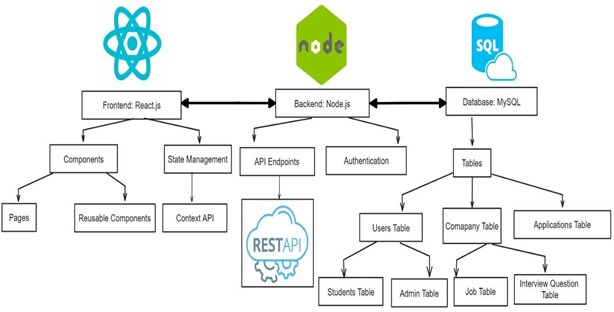
\includegraphics[width=0.9\textwidth]{Images/Picture1.jpg} % change filename here
    \caption{System Architecture}
\end{figure}
Fig. 5.1 showcases the high-level architectural design of HireStream. The diagram illustrates the flow of data from the user interface in the frontend to the backend services, and then to the database. It highlights the integration of AI components for functionalities such as job recommendations and resume parsing, along with the role of the API Gateway in routing and securing communications.

\section{Use-Case Diagram}
\noindent The use-case diagram outlines interactions between the system’s actors:
\begin{itemize}[itemsep=-4pt]
    \item \textbf{Students}: Register, log in, search jobs, apply for jobs, track application status, and interact with alumni.
    \item \textbf{Recruiters}: Post jobs, manage applications, and schedule interviews
    \item \textbf{Placement Officers}: Oversee job postings, manage student applications, and generate reports.
\end{itemize}
\begin{figure}[h!]
    \centering
    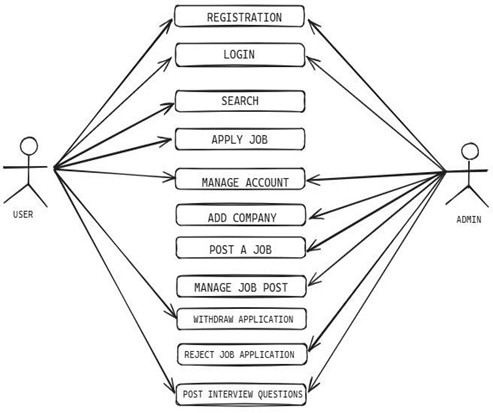
\includegraphics[width=0.9\textwidth]{Images/Picture2.jpg} % change filename here
    \caption{Use-Case Diagram}
\end{figure}
The use case diagram illustrates the interaction between the User and Admin within the job placement system. The User can perform essential activities such as registration, login, searching for jobs, applying for jobs, and managing their account. The User is also able to withdraw their application if needed. The Admin, on the other hand, holds responsibilities related to managing the platform, such as adding companies, posting job openings, and managing job posts. The Admin can also review applications and either accept or reject them based on eligibility criteria. 
\pagebreak


Fig. 5.2 visually maps the relationships between the system actors and their activities, demonstrating the full scope of user interactions. It illustrates specific actions such as "post jobs" for recruiters and "apply for jobs" for students, showing the interactions with backend systems for each use case.
\section{Dataflow Diagram}
\noindent The dataflow diagram depicts the relationships between system entities:
\begin{itemize}[itemsep=-4pt]
    \item \textbf{User}: Attributes like name, role (student/recruiter), and login details.
    \item \textbf{Job}: Includes details such as title, description, eligibility, and company.
    \item \textbf{Application}: Tracks the status of each job application by users
\end{itemize}

\begin{figure}[h!]
    \centering
    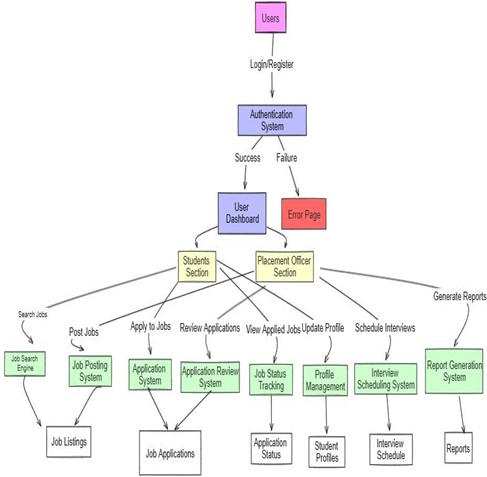
\includegraphics[width=0.9\textwidth]{Images/Picture3.jpg} % change filename here
    \caption{Dataflow Diagram}
\end{figure}
\noindent The Data Flow Diagram illustrates the flow of user interactions within the placement management system. Users first authenticate through the Authentication System, which either grants access to the User Dashboard or redirects to an error page upon failure. From the dashboard, students and placement officers navigate to their sections to perform tasks.
\pagebreak

Fig. 5.3 provides a detailed representation of the system's data structure. It shows how users relate to jobs and applications, emphasizing the attributes and methods that enable functionalities such as profile updates and application tracking.



\chapter{Implementation}

This chapter discusses the step-by-step implementation of the project titled "HireStream The Next-Gen Job Portal with Integrated Interviews and AI Assistance"

\section{Implementation details of the modules}
\noindent \textbf{Module 1:Frontend(React and vite)}
\begin{itemize}[itemsep=-4pt]
    \item The frontend of the system is developed using React with Vite, a modern build tool known for its speed and efficient development workflow. The frontend provides an intuitive and responsive user interface for interacting with the HireStream application. The key functionalities of the frontend module include:
    \item \textbf{User Dashboard}: Provides users, colleges, and companies with a streamlined dashboard for managing profiles, applications, and job postings.
    \item \textbf{Role-based Access}: Enables colleges to assign permissions to placement staff and department staff to customize jobs and user verification.
    \item \textbf{Job Management}: Includes features for posting, editing, and managing job listings with rich text formatting.
    \item \textbf{Visualization and Analytics}: Implements dynamic charts and data visualizations using libraries like React Circular Progress Bar and @tanstack/react-table to display application trends and user activity.
    \item \textbf{	Authentication and Security}: Incorporates Firebase for secure user authentication and Redux Persist for state management across sessions.
    \item \textbf{Responsive Design}: Uses Tailwind CSS and ShadCN/UI for creating an accessible and responsive design across devices.
\end{itemize}
\noindent \textbf{Module 2:Data Processing and Management}
\begin{itemize}[itemsep=-4pt]
    \item The Data Processing Module is responsible for handling job applications, user profiles, and other critical data, ensuring they are processed and stored efficiently in the database. Key operations include:
    \item \textbf{Data Validation}: Ensures input data, such as job descriptions, user profiles, and applications, meets defined standards before processing.
    \item \textbf{Media Management}: Manages uploads like profile images or job-related files using Multer and stores them securely on Cloudinary.
    \item 	\textbf{Data Transformation}: Converts raw input data into a normalized format, enabling seamless integration with the backend.
    \item \textbf{Integration with MongoDB}: Utilizes Drizzle ORM for a type-safe and optimized interaction with the NeonDB-hosted MongoDB database

\end{itemize}
\noindent \textbf{Module 3:Backend Services(Node.js and MongoDB}
\begin{itemize}[itemsep=-4pt]
    \item The backend is developed using Node.js and handles business logic, database interactions, and APIs. Key functionalities include:
    \item 	\textbf{Role-based Access Control (RBAC)}: Implements secure access control for different user roles ( department staff, placement staff, student) using JSON Web Tokens (JWT).
    \item\textbf{	Job and Application APIs}: Provides RESTful endpoints for managing job postings, applications, and user profiles using Express.
    \item \textbf{Database Management}: Uses Drizzle ORM to interact with a MongoDB database hosted on NeonDB, ensuring efficient and secure data operations.

    \item 	\textbf{Password Security}: Incorporates bcryptjs for hashing passwords and enhancing user security.
    \item \textbf{File Management}: Uses Cloudinary for hosting and retrieving media files uploaded by users.
    \item \textbf{Session Management}: Uses cookie-parser for managing user sessions securely.
\end{itemize}
\section{\textbf{Pseudo Code for Pre-Processing Techniques}}
\subsection{\textbf{Frontend Program (Admin Portal)}}

This code represents the main routing and navigation logic of the HireStream web application built using React. It uses React Router to manage page navigation and Redux to access the authenticated user state. Based on the user’s login status, the application conditionally renders either the dashboard or the home page. Protected routes are implemented using custom components such as Authenticated Routes and Admin Route to ensure role-based access control. The Dashboard component acts as a layout wrapper for all authenticated pages. Dynamic routing is used to display job and company details using URL parameters. Separate routes are defined for posting jobs and companies, accessible only to authorized users. The application also includes verification, user profile, and account management routes. A 'ScrollToTop' component ensures smooth navigation between pages. Overall, this routing structure ensures secure, organized, and user-friendly navigation across the HireStream platform.


\noindent \begin{lstlisting}
import { useSelector } from "react-redux";
import { BrowserRouter, Navigate, Route, Routes } from "react-router-dom";
import AdminRoute from "./components/non-shadcn/AdminRoute";
import AuthenticatedRoutes from "./components/non-shadcn/AuthenticatedRoute";
import ScrollToTop from "./components/non-shadcn/ScrollToTop";
import Account from "./pages/Account";
import Companies from "./pages/Companies";
import Dashboard from "./pages/Dashboard";
import Forms from "./pages/Forms";
import Home from "./pages/Home";
import Jobs from "./pages/Jobs";
import PostCompany from "./pages/PostCompany";
import PostJob from "./pages/PostJob";
import SignIn from "./pages/SignIn";
import SignUp from "./pages/SignUp";
import User from "./pages/User";
import Verification from "./pages/Verification";
import Company from "./pages/Company";
export default function App() {
const { currentUser: user } = useSelector((state) => state.user);
return (
<BrowserRouter>
<ScrollToTop />
<Routes>
{user ? (
<Route element={<Dashboard user={user} />}>
<Route path="/" element={
<div className="flex flex-col items-center justify-center min-h-screen bg-gradient-to-br from-blue-50 to-blue-100 dark:from-gray-900 dark:to-gray-800 text-gray-800 dark:text-gray-100 p-4 transition-colors duration-300">
<div className="text-center bg-white dark:bg-gray-700 shadow-2xl dark:shadow-xl rounded-xl p-12 transform transition duration-500 hover:scale-105">
<h1 className="text-5xl font-bold tracking-tight mb-4 text-blue-800 dark:text-blue-300 drop-shadow-md">
Hi, {user.name}
</h1>
<p className="text-xl font-medium text-gray-600 dark:text-gray-300 opacity-90 animate-pulse">
Welcome to Hire Stream Admin Portal
</p>
</div>
<div className="absolute bottom-10 opacity-50 dark:opacity-40">
<svg xmlns="http://www.w3.org/2000/svg" width="100" height="50" viewBox="0 0 100 50" className="animate-bounce">
<path d="M10 15 L50 40 L90 15" fill="none" stroke="#1E40AF" className="dark:stroke-blue-500" strokeWidth="4" strokeLinecap="round"/>
</svg>
</div>
</div>
}
/>
<Route element={<AuthenticatedRoutes />}>
<Route path="jobs" element={<Jobs />}>
<Route path=":jobId" element={<div>Job Details</div>} />
</Route>
<Route path="companies" element={<Companies userRole={user.role} />}>
<Route path=":companyId" element={<Company />} />
</Route>
<Route path="forms" element={<AdminRoute />}>
<Route path="" element={<Forms />} />
<Route path="company" element={<PostCompany />} />
<Route path="job" element={<PostJob user={user} />} />
</Route>
<Route path="/verify" element={<Verification verify={true} />} />
<Route path="/team" element={<Verification verify={false} />} />
</Route>
<Route path="/user" element={<div className="grid gap-4 md:grid-cols-3">users</div>} />
<Route path="/user/:userId" element={<User user={user} />} />
<Route path="/account" element={<Account />} />
</Route>
) : (
<Route path="/" element={<Home />} />
)}
<Route path="/sign-in" element={user ? <Navigate to="/" /> : <SignIn />} />
<Route path="/sign-up" element={user ? <Navigate to="/" /> : <SignUp />} />
</Routes>
</BrowserRouter>
);
}
\end{lstlisting}

\subsection{\textbf{Frontend Program (Student Portal)}}

This code defines the main routing structure for the HireStream Student Portal using React. It utilizes Redux to fetch the currently logged-in user and React Router to manage application navigation. A global Web cam context is created to control web cam access for mock interview features. The application conditionally renders routes based on the user’s authentication status. Once logged in, users are redirected to a dashboard that serves as a common layout for all student pages. The home route displays a personalized welcome screen with the student’s name. Protected routes are handled using the Authenticated Routes component to restrict unauthorized access. The routing includes modules for jobs, companies, user profiles, and account management. The Toaster component is used to display real-time notifications. Overall, this structure ensures secure, organized, and interactive navigation within the HireStream student interface.

\noindent \begin{lstlisting}
import { useSelector } from "react-redux";
import { BrowserRouter, Navigate, Route, Routes } from "react-router-dom";
import AuthenticatedRoutes from "./components/non-shadcn/AuthenticatedRoute";
import ScrollToTop from "./components/non-shadcn/ScrollToTop";
import Account from "./pages/Account";
import Companies from "./pages/Companies";
import Dashboard from "./pages/Dashboard";
import Home from "./pages/Home";
import Jobs from "./pages/Jobs";
import SignIn from "./pages/SignIn";
import SignUp from "./pages/SignUp";
import User from "./pages/User";
import { Toaster } from "./components/ui/toaster";
import Interview from "./components/non-shadcn/mockInterview/Interview";
import { createContext, useState } from "react";
import StartInterview from "./components/non-shadcn/mockInterview/StartInterview";
import Company from "./pages/Company";
export const WebCamContext = createContext();
export default function App() {
const { currentUser: user } = useSelector((state) => state.user);
const [webCamEnabled, setWebCamEnabled] = useState(false);
return (
<WebCamContext.Provider value={{ webCamEnabled, setWebCamEnabled }}>
<BrowserRouter>
<ScrollToTop />
<Toaster />
<Routes>
{user ? (
<Route element={<Dashboard user={user} />}>
<Route path="/" element={
<div className="flex flex-col items-center justify-center min-h-screen bg-gradient-to-br from-blue-50 to-blue-100 dark:from-gray-900 dark:to-gray-800 text-gray-800 dark:text-gray-100 p-4 transition-colors duration-300">
<div className="text-center bg-white dark:bg-gray-700 shadow-2xl dark:shadow-xl rounded-xl p-12 transform transition duration-500 hover:scale-105">
<h1 className="text-5xl font-bold tracking-tight mb-4 text-blue-800 dark:text-blue-300 drop-shadow-md">
Hi, {user.name}
</h1>
<p className="text-xl font-medium text-gray-600 dark:text-gray-300 opacity-90 animate-pulse">
Welcome to Hire Stream Student Portal
</p>
</div>
<div className="absolute bottom-10 opacity-50 dark:opacity-40">
<svg xmlns="http://www.w3.org/2000/svg" width="100" height="50" viewBox="0 0 100 50" className="animate-bounce">
<path d="M10 15 L50 40 L90 15" fill="none" stroke="#1E40AF" className="dark:stroke-blue-500" strokeWidth="4" strokeLinecap="round"/>
</svg>
</div>
</div>
}
/>

\end{lstlisting}
\section{\textbf{Backend Program}}

This code represents the backend server setup of the HireStream application developed using Node.js and Express.js. The Express framework is used to create a RESTful API for handling client requests efficiently. CORS middleware is configured to allow secure communication between the frontend and backend during development. Environment variables are managed using dotenv to improve security and flexibility. The application connects to a database through a dedicated database configuration module. Separate route handlers are defined for users, recruiters, admins, students, and job applications to maintain modularity. Each router manages its respective API endpoints and business logic. Middleware is used to parse JSON and URL encoded data from incoming requests. A default route is added to verify that the server is running successfully. Overall, this backend architecture ensures scalability, security, and organized request handling for the HireStream platform.

\noindent \begin{lstlisting}
import express from 'express';
import cors from 'cors';
import UserRouter from './Routes/User.router.js';
import RecruiterRouter from './Routes/Recruiter.router.js';
import db from './config/db.js';
import AdminRouter from './Routes/Admin.router.js';
import StudentRouter from './Routes/Student.routes.js';
import ApplicationRouter from './Routes/Application.routes.js';
import dotenv from 'dotenv';
dotenv.config();
const app = express();
app.use(
  cors({
    origin: 'http://localhost:5173',
    methods: ['GET', 'POST', 'PUT', 'DELETE', 'PATCH', 'OPTIONS'],
    allowedHeaders: ['Content-Type', 'Authorization'],
  })
);
app.use(express.json());
app.use(express.urlencoded({ extended: true }));
const port = process.env.PORT || 5000;
db();
app.use('/user', UserRouter);
app.use('/recruiter', RecruiterRouter);
app.use('/admin', AdminRouter);
app.use('/student', StudentRouter);
app.use('/applications', ApplicationRouter);
app.get('/', (req, res) => {
  res.status(200).send({ message: 'server started' });
});
app.listen(port, () => {
  console.log(`Server running on http://localhost:${port}`);
});

\end{lstlisting}

\section{\textbf{Database Schema}}

This database schema defines the core relational structure of the HireStream platform using MongoDB. The users table stores comprehensive information about all registered users, including students, recruiters, and administrators, with unique identifiers, personal details, and authentication credentials. It maintains relationships with the colleges and branches tables through foreign key references to ensure data consistency and institutional mapping. User roles and verification status are managed to support role-based access and security. Academic details such as batch, CGPA, resume link, and profile description are included to support placement-related features. The branches table represents different academic departments and stores descriptive information for each branch. The colleges table maintains institutional details, including college names, descriptions, and logos. The companies table stores recruiter company information along with optional interview or assessment questions in JSON format. Overall, this schema ensures normalized data storage, referential integrity, and scalability for managing users, institutions, and recruitment entities efficiently.

\noindent \begin{lstlisting}
export const users = pgTable("users", {
  uid: varchar("uid", { length: 20 }).primaryKey(),
  name: varchar("name", { length: 255 }).notNull(),
  email: varchar("email", { length: 255 }).unique().notNull(),
  password: varchar("password", { length: 255 }).notNull(),
  dob: date("dob").notNull(),
  phoneNo: bigint("phone_no", { mode: "number" }).unique().notNull(),
  collegeId: varchar("college_id", { length: 20 })
    .notNull()
    .references(() => colleges.collegeId),
  branchId: varchar("branch_id", { length: 20 })
    .references(() => branches.branchId),
  role: varchar("role", { length: 255 }).default("student").notNull(),
  verified: boolean("verified").notNull().default(false),
  batch: varchar("batch", { length: 255 }),
  cgpa: real("cgpa"),
  resumeLink: varchar("resume_link", { length: 1024 }),
  description: text("description"),
  profileImageUrl: varchar("profile_image_url", { length: 1024 }).default(
    "https://cdn-icons-png.flaticon.com/512/9512/9512683.png"
  ),
});
export const branches = pgTable("branches", {
  branchId: varchar("branch_id", { length: 20 }).primaryKey().notNull(),
  name: varchar("name", { length: 255 }).notNull(),
  description: text("description"),
});
export const colleges = pgTable("colleges", {
  collegeId: varchar("college_id", { length: 20 }).primaryKey().notNull(),
  name: varchar("name", { length: 255 }).notNull(),
  description: text("description"),
  logoUrl: varchar("logo_url", { length: 1024 }),
});
export const companies = pgTable("companies", {
  id: serial("id").primaryKey(),
  companyId: varchar("company_id", { length: 20 }).unique().notNull(),
  questions: jsonb("questions", { length: 1024 }),
});
\end{lstlisting}




\chapter{Results and Discussion}

The Results chapter of this report presents an overview of HireStream's performance, demonstrating its functionality through snapshots of the platform. These snapshots illustrate key features such as user registration, job postings, candidate applications, and administrative controls.

\section{\textbf{Snapshots}}
\subsection{Student Portal}
\begin{figure}[h!]
    \centering
    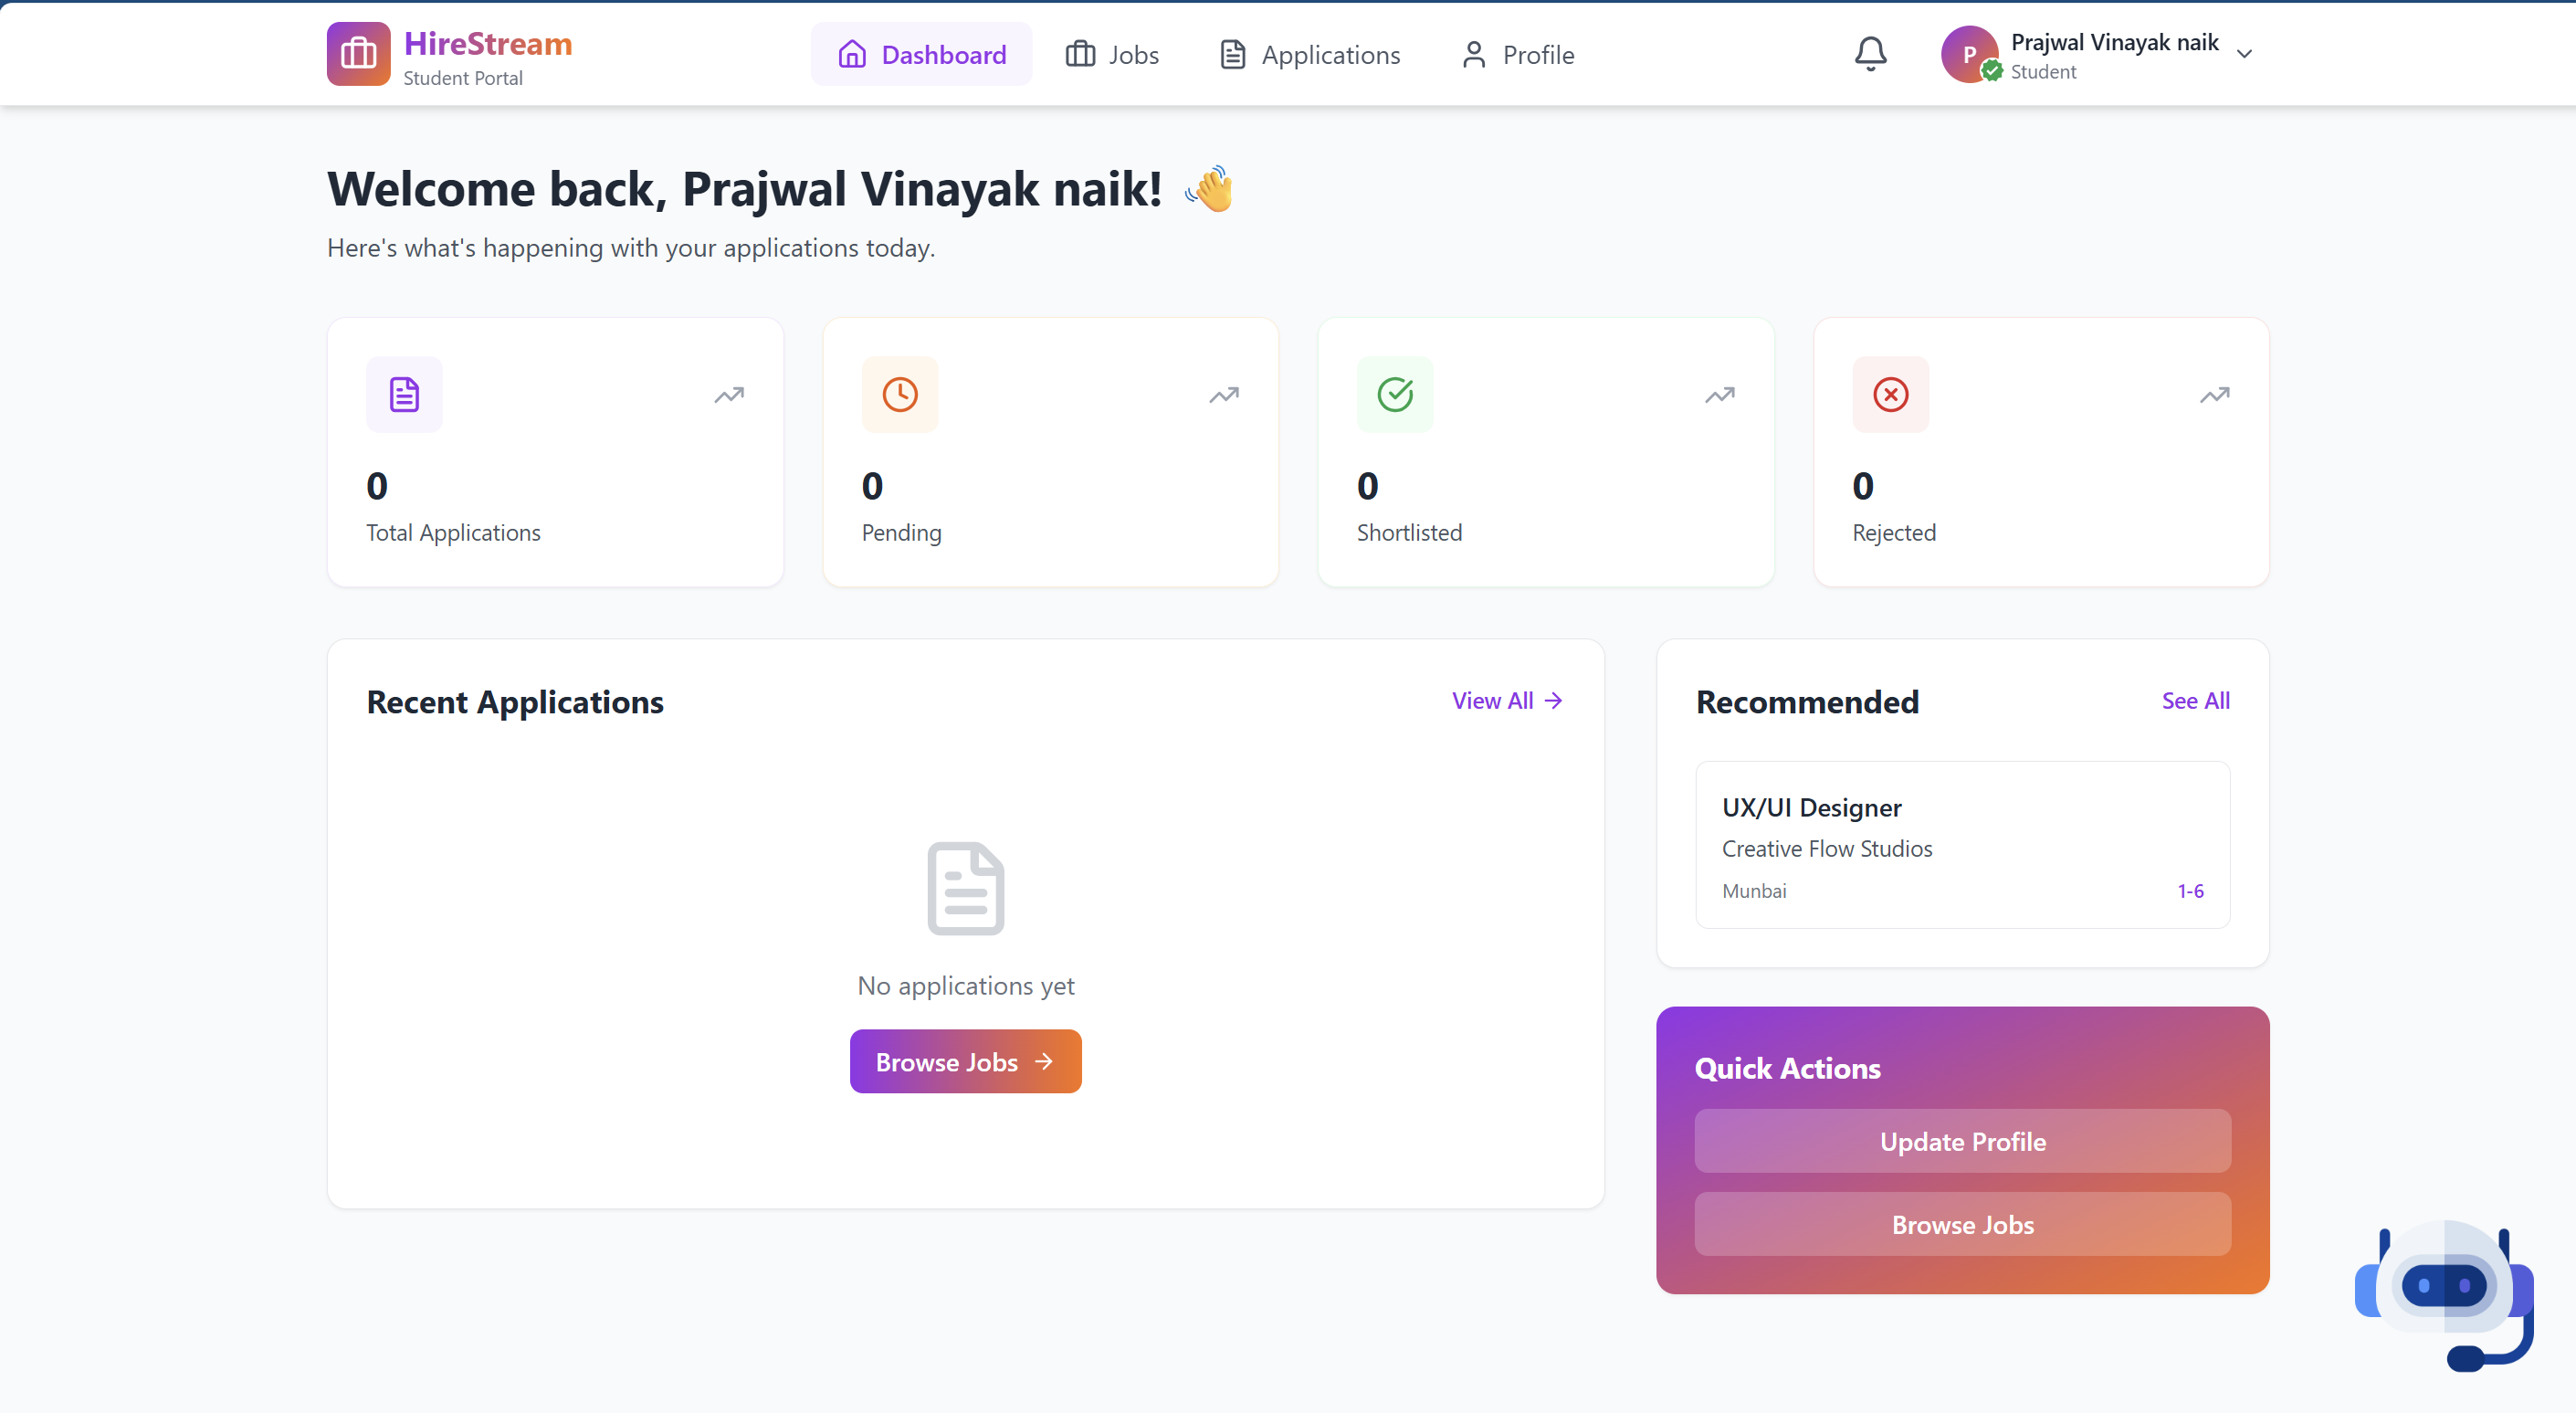
\includegraphics[width=0.9\textwidth]{Images/Screenshot_1.png} % change filename here
    \caption{Student Portal}
\end{figure}
Fig. 7.1 student portal provides an organized and user-friendly interface for students to manage their placement activities. Students can browse available job opportunities, track their application status, and update their profile information. The dashboard offers quick access to interviews, assessments, and mock interview practice modules. Overall, the portal ensures a seamless and guided experience throughout the placement process.It also displays personalized greetings and important notifications to keep students updated. Navigation is simple and well-structured, allowing students to move between features without confusion.
\pagebreak
\subsection{Admin Portal}
\begin{figure}[h!]
    \centering
    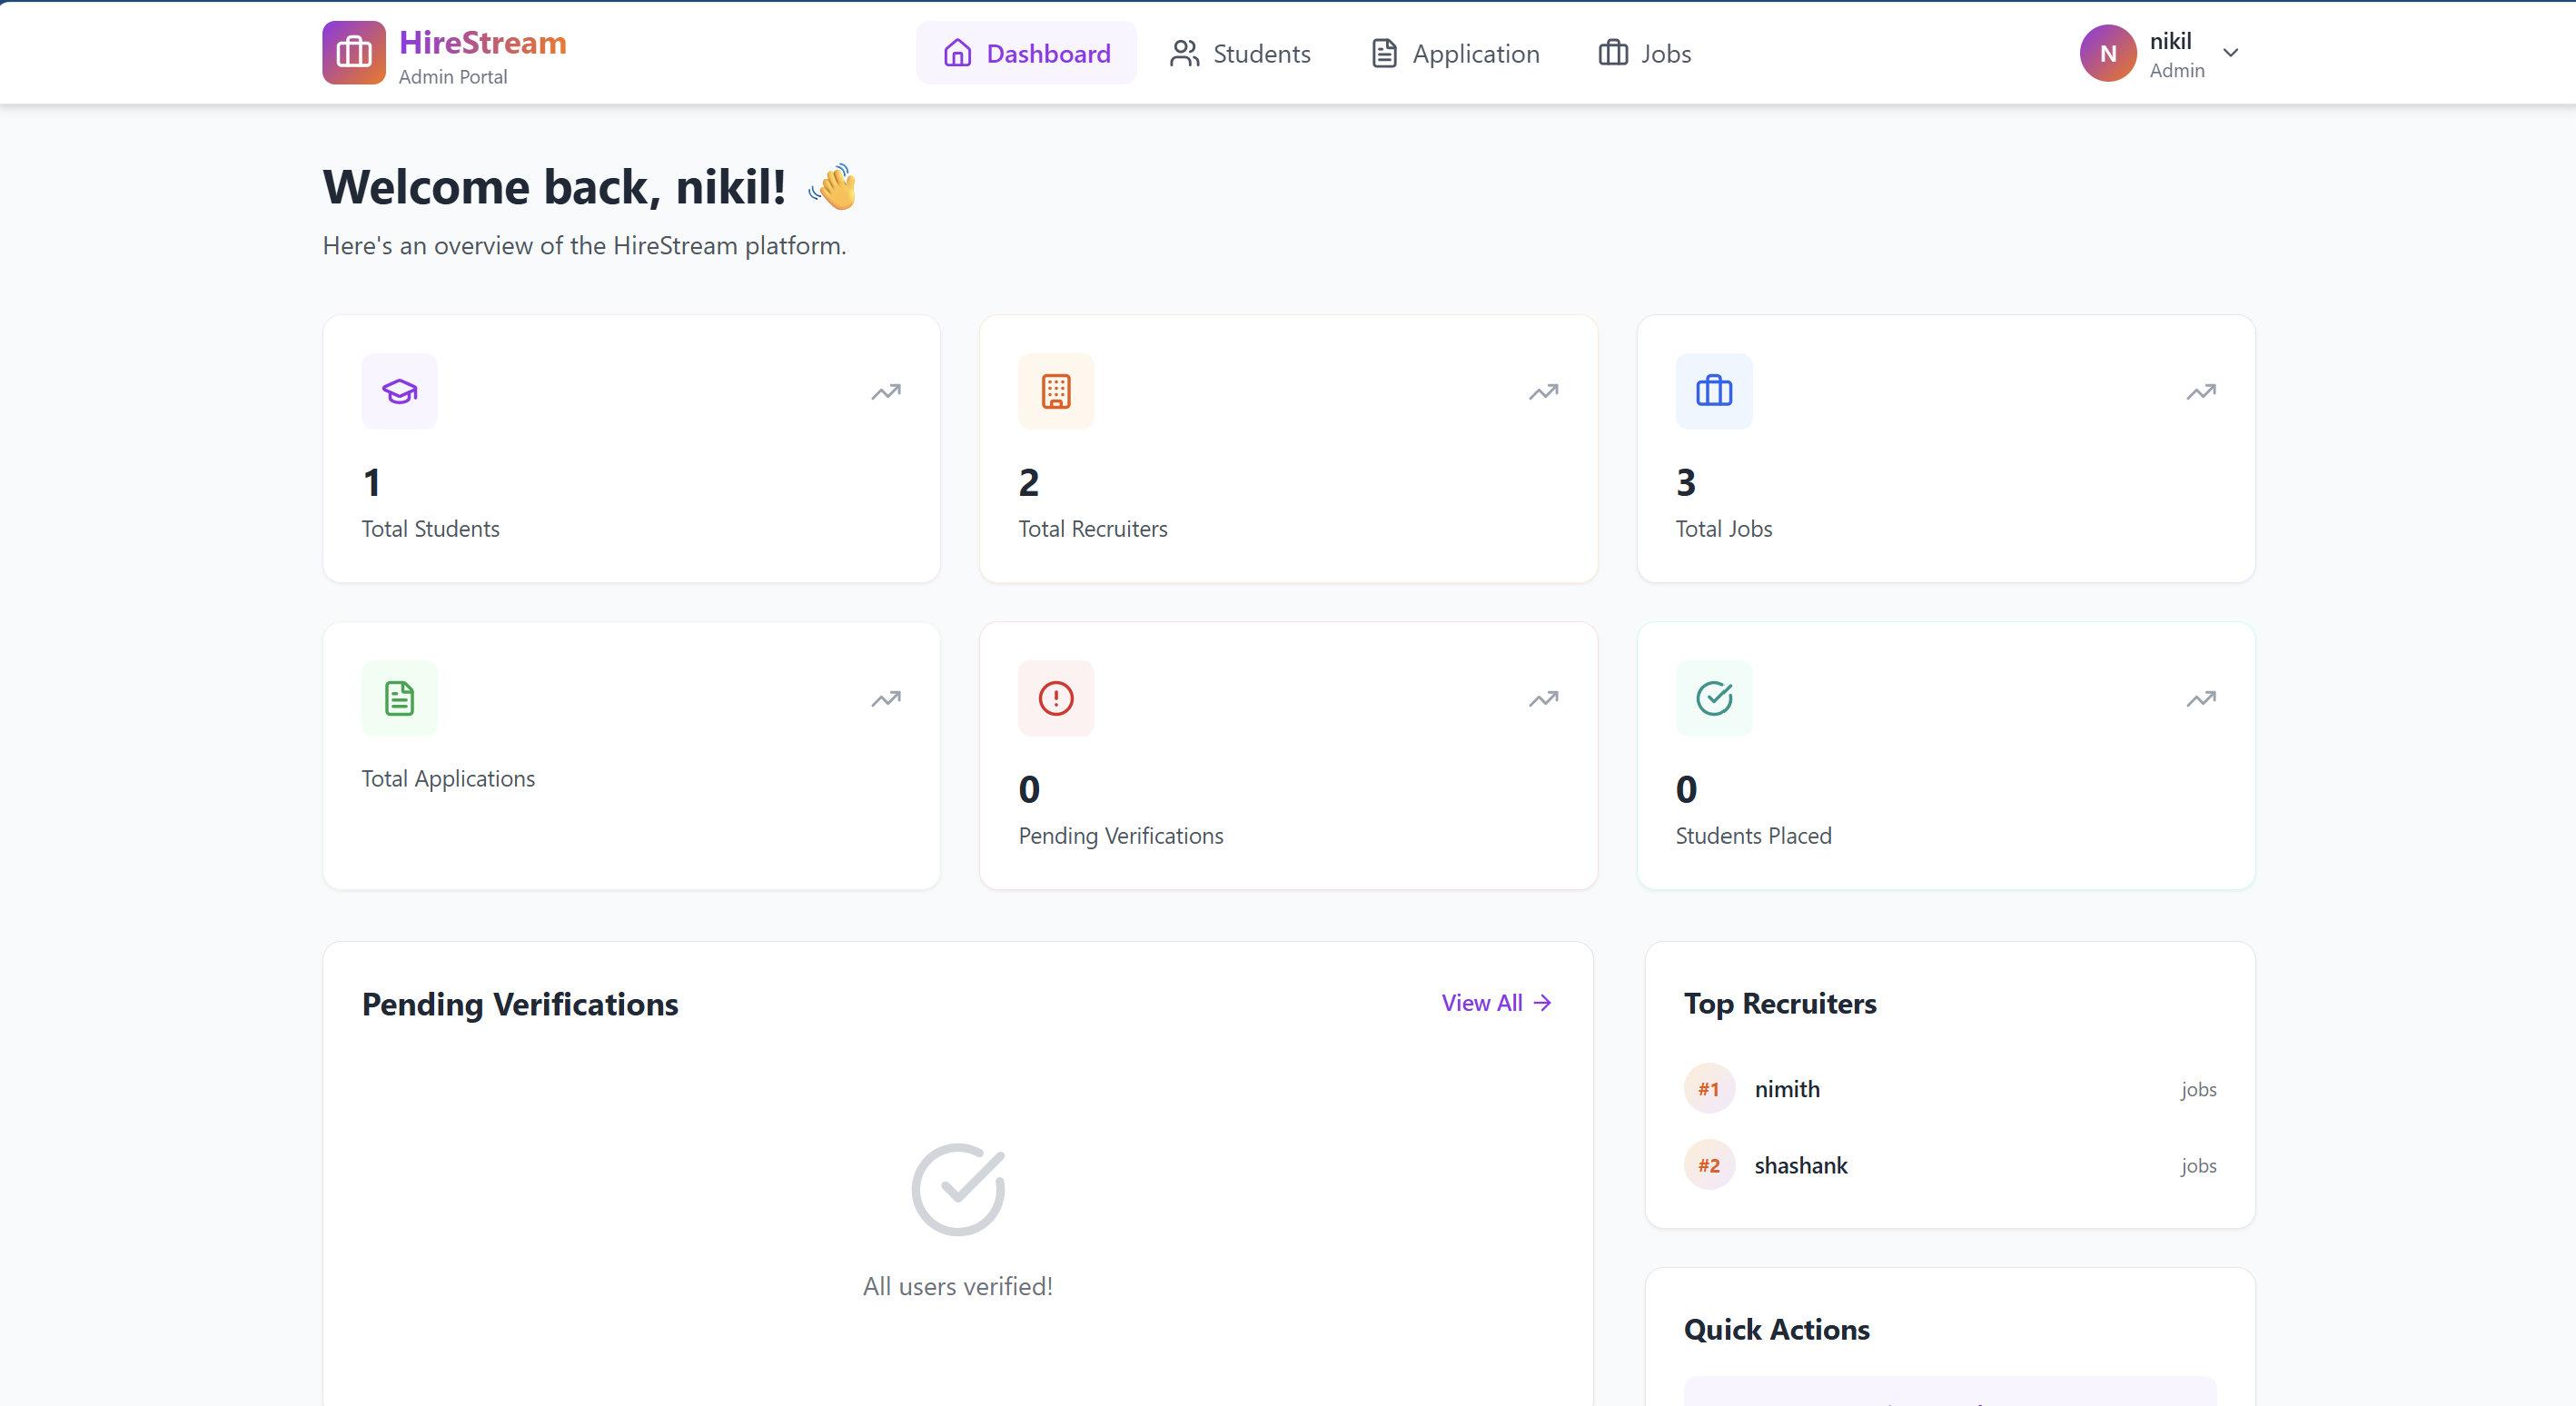
\includegraphics[width=0.9\textwidth]{Images/Screenshot2.png} % change filename here
    \caption{Admin Portal}
\end{figure}
Fig. 7.2 admin portal provides centralized control for managing all placement-related activities in the system. Administrators can add and manage companies, post job openings, and monitor student applications. It allows reviewing applicant details and updating their recruitment status, such as shortlisted, selected, or rejected. 

\subsection{Recruiter Portal}
\begin{figure}[h!]
    \centering
    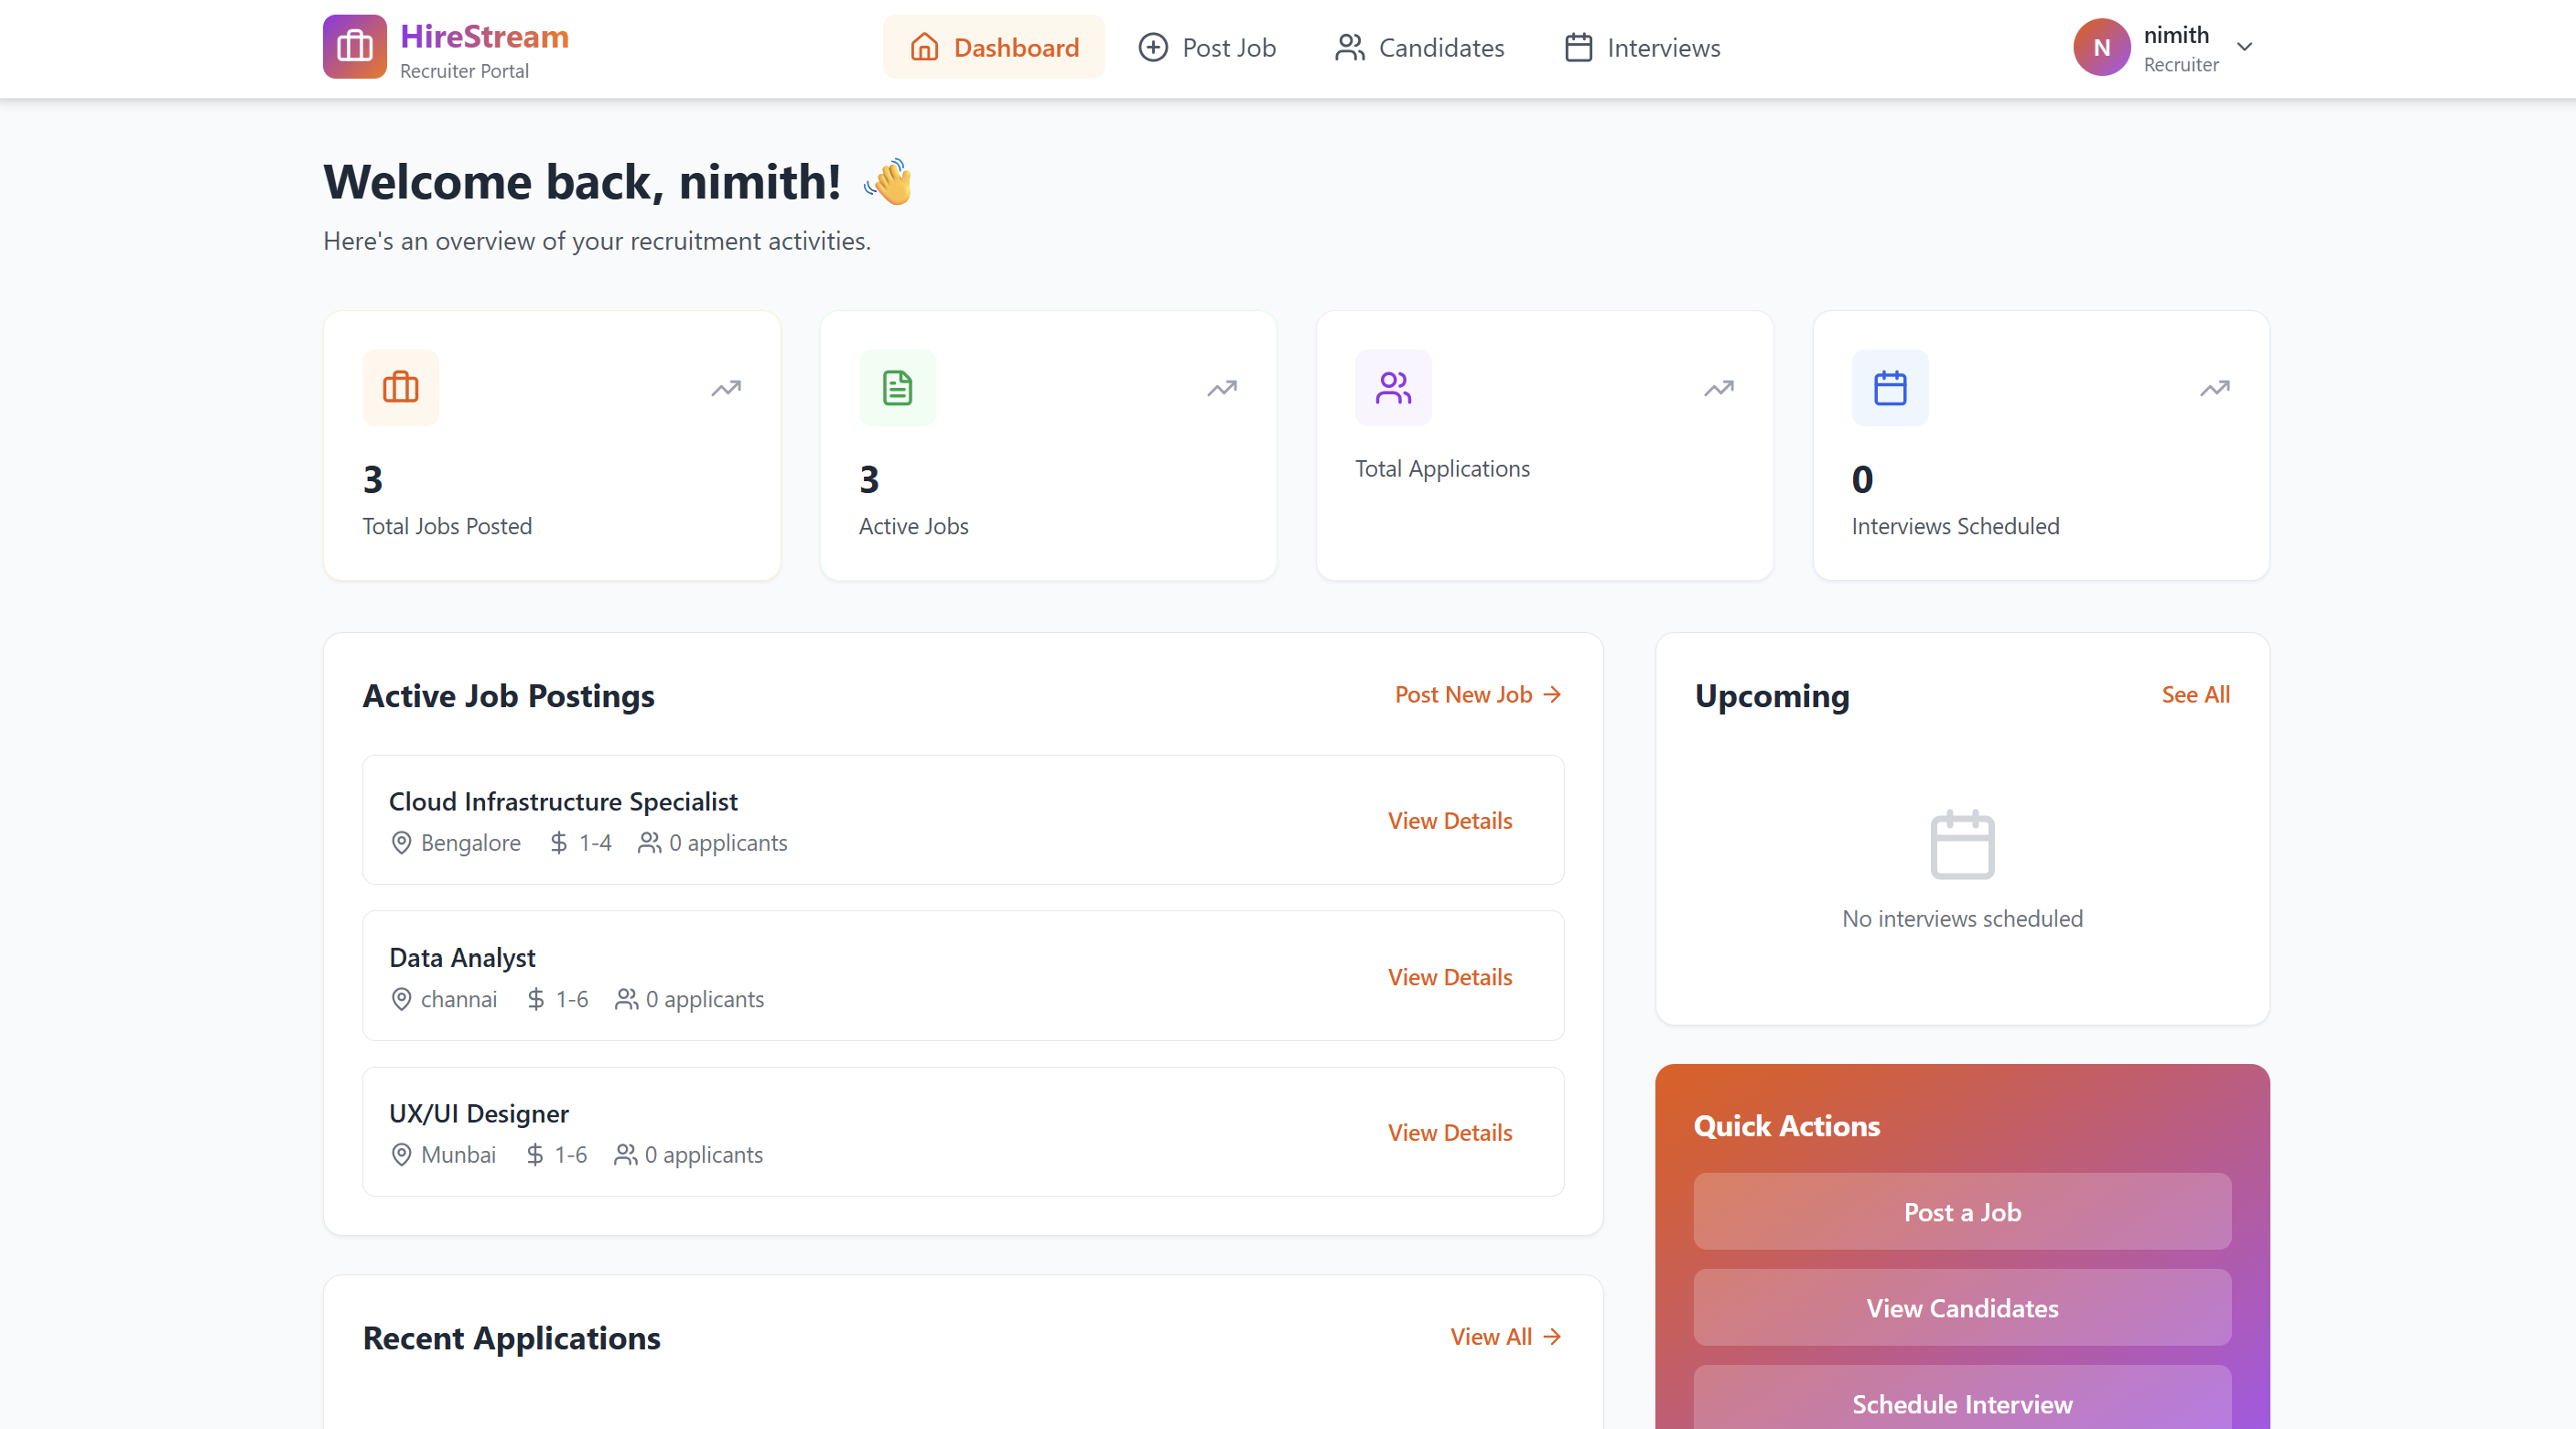
\includegraphics[width=0.9\textwidth]{Images/Screenshot3.png} % change filename here
    \caption{Recruiter Portal}
\end{figure}
Fig. 7.3 recruiter portal in the Hire Stream platform serves as a centralized system for companies to manage their hiring process seamlessly. It enables recruiters to post job openings, view applications, and shortlist candidates based on qualifications and skills. The portal offers a clear and intuitive interface, making it easy to track recruitment progress in real time. Recruiters can access detailed student profiles, including resumes and academic records, to make informed decisions.

\subsection{Student Profile}
\begin{figure}[h!]
    \centering
    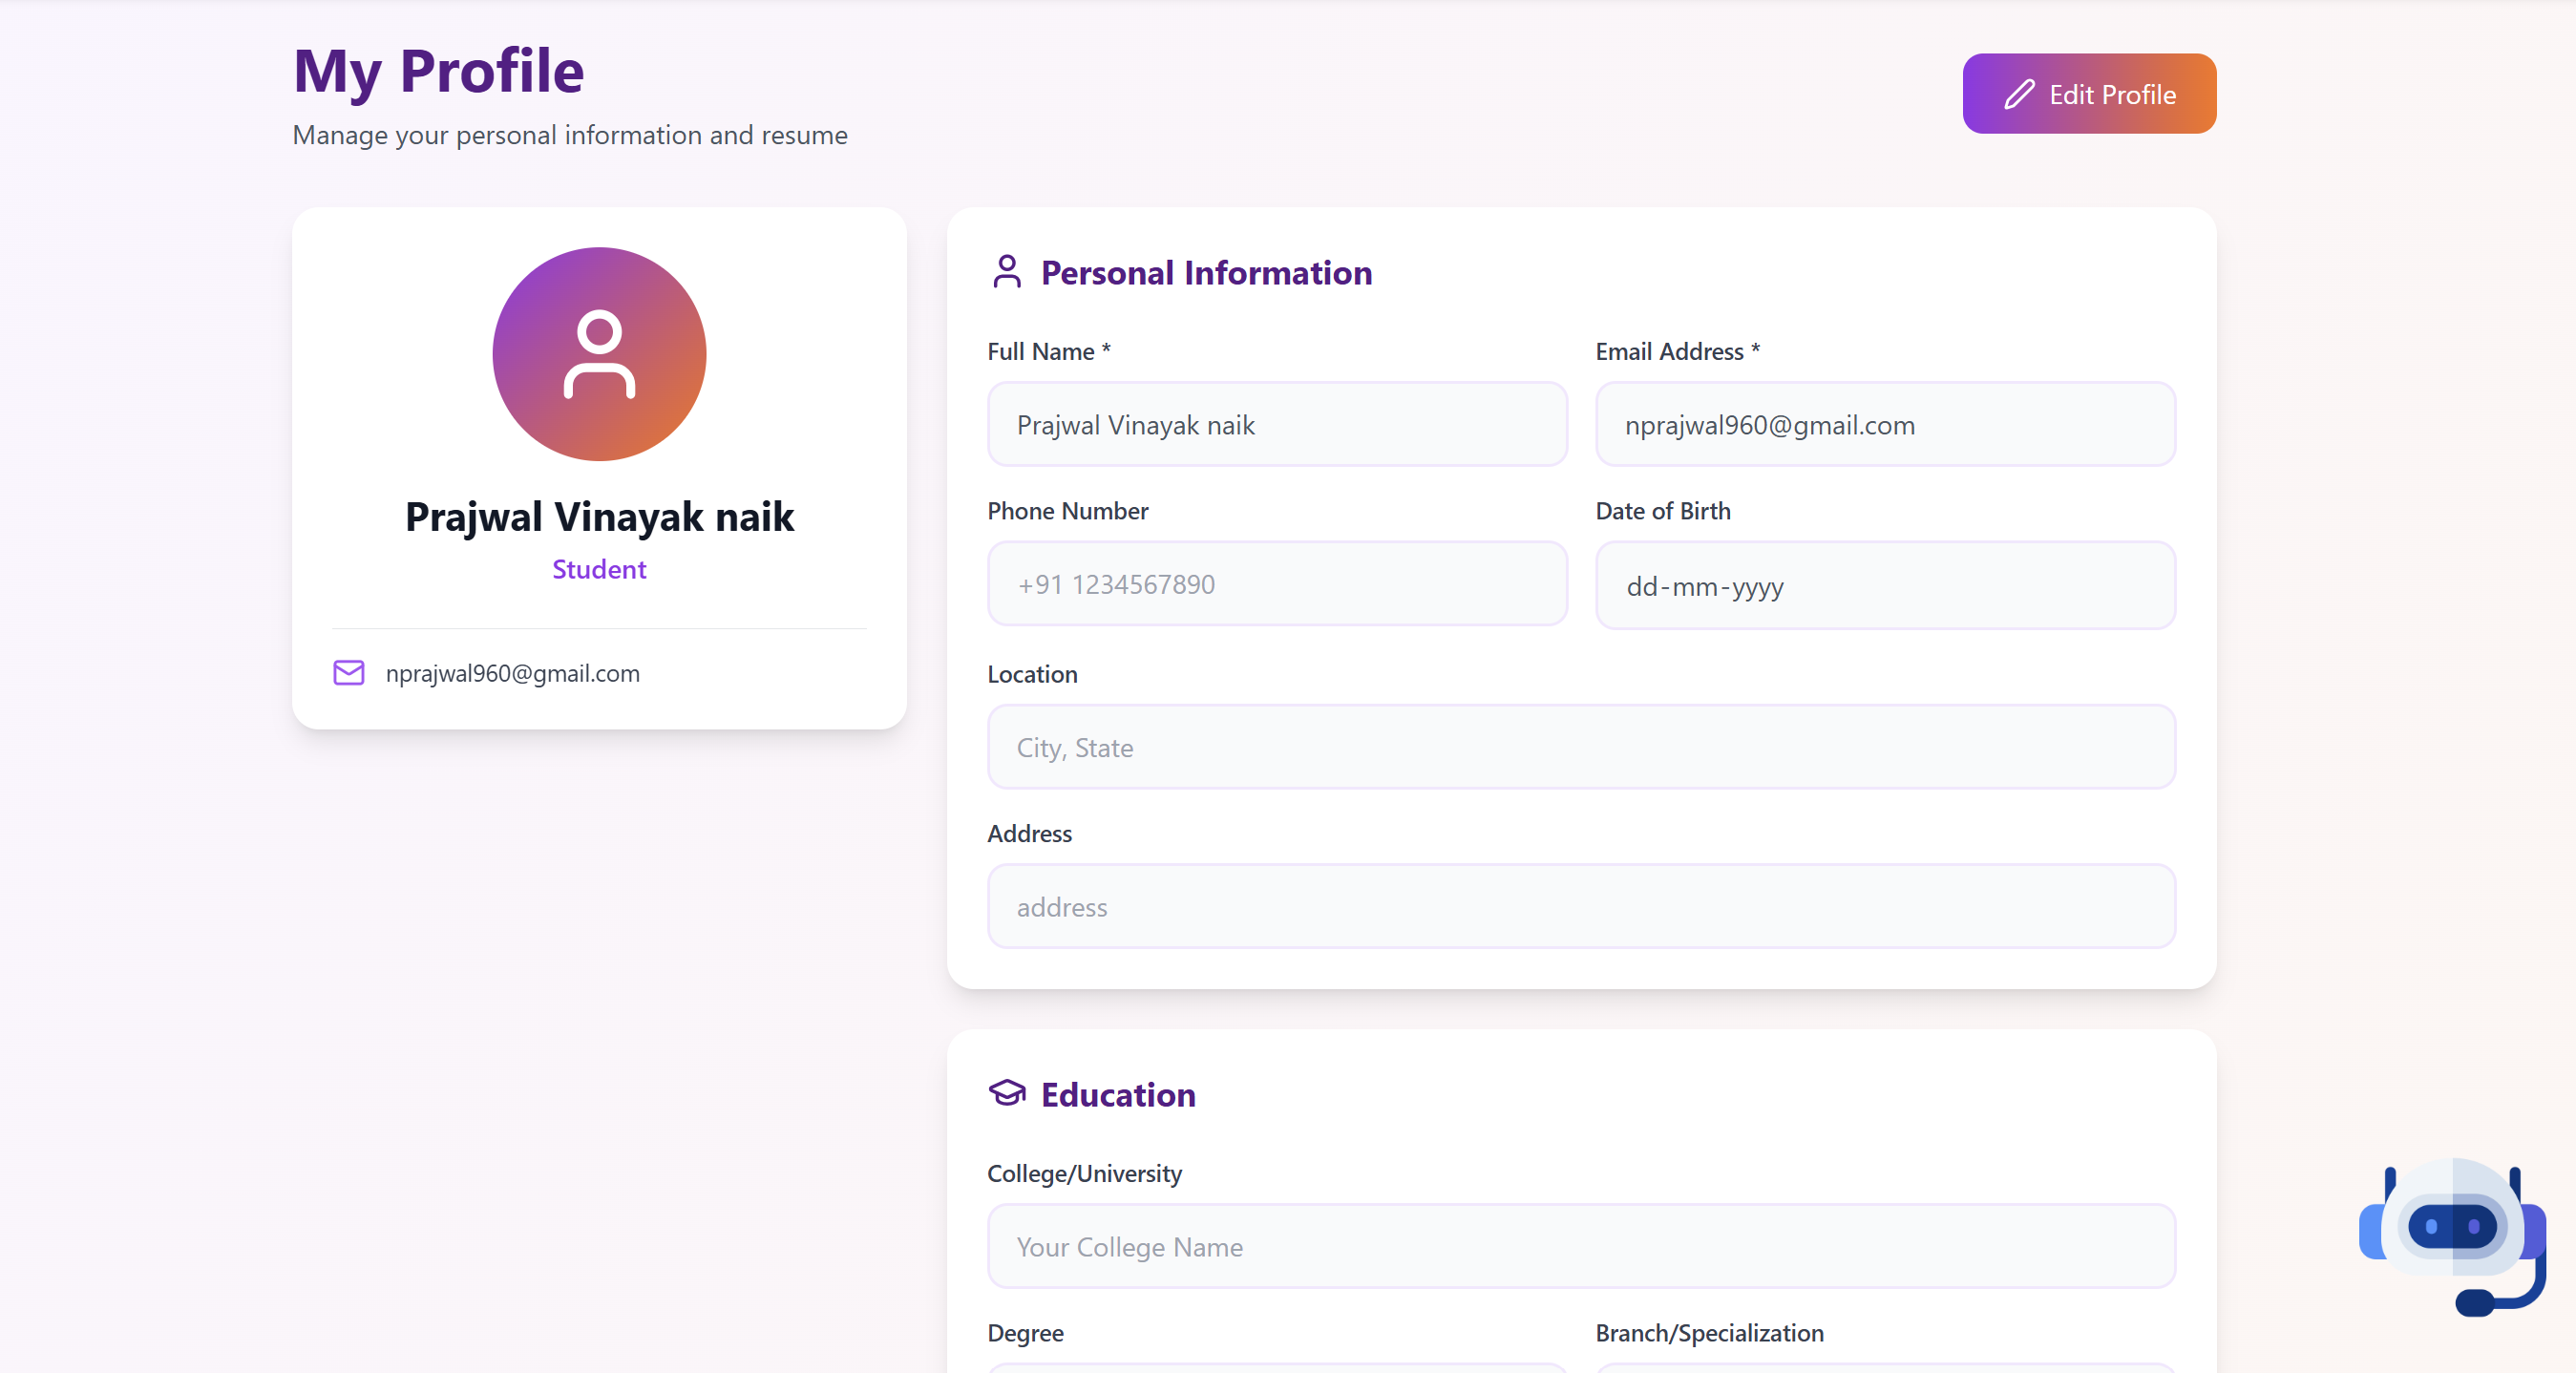
\includegraphics[width=0.9\textwidth]{Images/Screenshot4.png} % change filename here
    \caption{Student Profile}
\end{figure}
Fig. 7.4 student profile Page in the Hire Stream project provides a detailed overview of each student’s academic and professional information. It allows students to showcase their personal details, educational background, skills, and achievements in a structured format. The page includes sections for uploading resumes, certifications, and project links, giving recruiters a complete view of the candidate’s capabilities. Students can also update or edit their profiles to keep information current and accurate. The interface is designed to be simple, responsive, and visually organized for easy navigation. Recruiters can access these profiles to evaluate candidates and match them to suitable job roles. Overall, the page bridges the gap between students and recruiters by presenting all relevant details in one accessible and professional layout.

Additionally, the Student Profile Page includes an option to display internship experiences and extracurricular activities, helping recruiters assess overall personality and potential. It ensures data privacy and secure access, allowing only verified users.

\subsection{AI Chatbot Assistance}
\begin{figure}[h!]
    \centering
    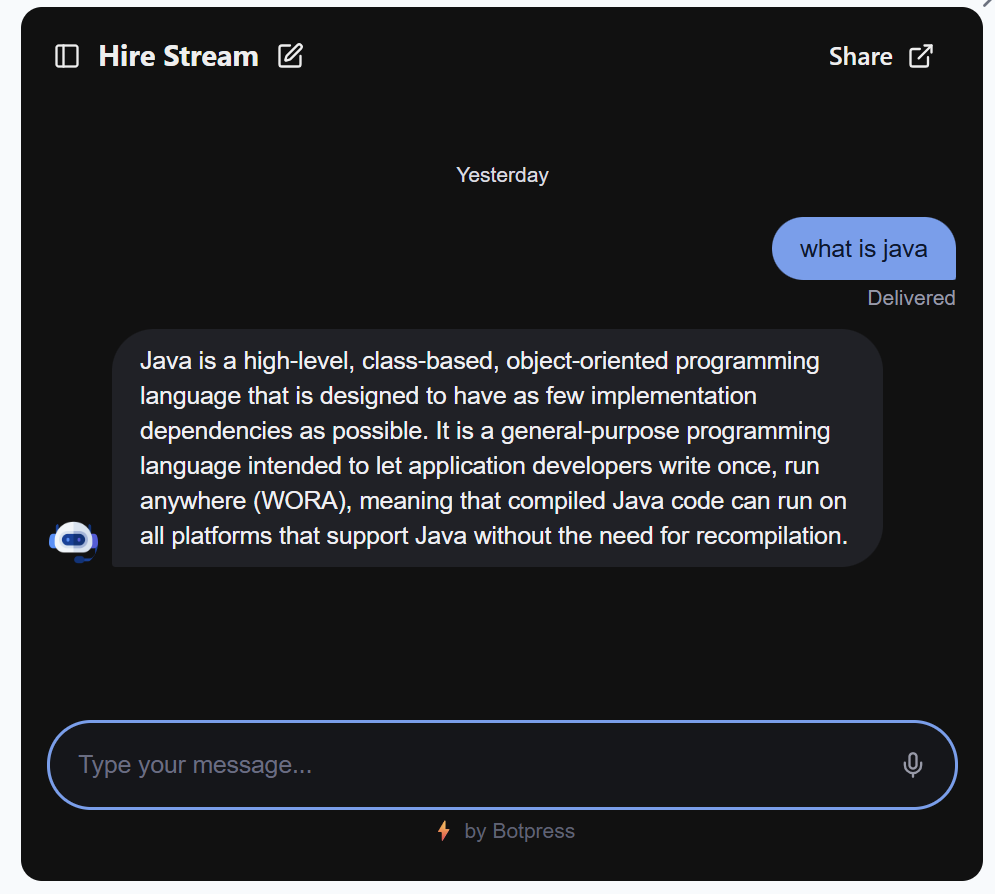
\includegraphics[width=0.9\textwidth]{Images/Screenshot5.png} % change filename here
    \caption{AI Chatbot Assistance}
\end{figure}
Fig. 7.5 AI Chatbot in the Hire Stream project acts as a virtual assistant to guide users throughout the platform. It helps students, recruiters, and admins by answering common queries and providing instant support related to profiles, job applications, and system navigation. The chatbot uses natural language processing (NLP) to understand user inputs and respond intelligently in real time. It enhances user engagement by offering personalized suggestions and quick solutions, reducing the need for manual support. Overall, the AI Chatbot improves the accessibility, efficiency, and interactivity of the Hire Stream platform.
\pagebreak
\section{Challenges and Limitations:}
Although the system performed well, some challenges were noted: 
\begin{itemize}[itemsep=-4pt]
    \item The system must ensure strong security to protect sensitive user data.

    \item Performance may reduce as the number of users and records increases.
    
    \item  The platform depends completely on stable internet connectivity.

    \item Advanced AI-based automation is limited in the current version.

    
\end{itemize}
\section{Summary}

The HireStream project successfully delivers a functional and reliable placement management system that meets its intended objectives. The platform enables smooth registration and authentication for students, recruiters, and administrators. Job postings, applications, and candidate shortlisting are handled efficiently through a centralized system. Users can easily track application status and receive timely notifications, improving transparency and communication. The system reduces manual effort in managing placement activities and minimizes data redundancy. Database integration ensures accurate storage and retrieval of user and recruitment information. Role-based access control enhances security and prevents unauthorized operations. The user interface is responsive and easy to use across devices. Overall, the project demonstrates effective integration of frontend, backend, and database components to support real-world placement workflows.


\chapter*{CO -- PO MAPPING}
\addcontentsline{toc}{chapter}{CO -- PO MAPPING}

\begin{center}
    {\Large \textbf{HireStream: The Next-Gen Job Portal with Integrated Interviews and AI Assistance}}
\end{center}

\vspace{0.6cm}

% ----------------------------------------------------------------
% SECTION i
% ----------------------------------------------------------------
\section*{i. CO/PSO Covered for Project Phase II with Justification}

\renewcommand{\arraystretch}{1.3}
\begin{tabular}{|c|p{12cm}|}
\hline
\textbf{CO1} & Apply engineering and computational knowledge to design modern job-portal systems with AI-driven features. \\ \hline
\textbf{CO2} & Develop innovative and feasible software solutions integrating job search, automated interviews, and AI assistance. \\ \hline
\textbf{CO3} & Plan, execute, and manage full-stack development tasks within defined timelines, ensuring secure and scalable deployment. \\ \hline
\textbf{CO4} & Communicate technical outputs effectively through UI/UX designs, analytics dashboards, and documentation. \\ \hline
\textbf{CO5} & Work effectively in teams to build modular job-portal components including authentication, ATS, AI interview engine, and analytics. \\ \hline
\textbf{CO6} & Demonstrate ethical, privacy-aware, and socially responsible design practices in handling applicant data and AI-based decision systems. \\ \hline
\end{tabular}


\vspace{1cm}

% ----------------------------------------------------------------
% SECTION ii
% ----------------------------------------------------------------
\section*{ii. CO--PO/PSO Mapping Table}

\renewcommand{\arraystretch}{1.3}
\setlength{\tabcolsep}{6pt}

\begin{table}[h!]
\centering
\resizebox{\textwidth}{!}{
\begin{tabular}{|c|c|c|c|c|c|c|c|c|c|c|c|c|c|}
\hline
\textbf{COs} & \textbf{PO1} & \textbf{PO2} & \textbf{PO3} & \textbf{PO4} & \textbf{PO5} & \textbf{PO6} & \textbf{PO7} & \textbf{PO8} & \textbf{PO9} & \textbf{PO10} & \textbf{PO11} & \textbf{PSO1} & \textbf{PSO2} \\ \hline

CO1 & 3 & 3 & 2 & 3 & 2 &   &   & 2 & 3 & 2 &   & 3 & 2 \\ \hline
CO2 & 3 & 3 & 3 & 2 & 3 &   &   & 2 & 2 & 2 &   & 3 & 3 \\ \hline
CO3 & 2 & 2 & 3 & 2 & 3 &   &   & 2 & 3 & 3 & 2 & 2 & 2 \\ \hline
CO4 & 2 & 2 & 2 & 3 & 3 &   &   & 3 & 2 & 3 & 2 & 2 & 2 \\ \hline
CO5 & 2 & 2 & 2 & 2 & 3 &   & 2 & 2 & 3 & 3 & 2 & 3 & 2 \\ \hline
CO6 & 2 &   &   & 2 & 2 & 3 & 3 & 3 & 2 & 2 &   & 2 & 3 \\ \hline

\textbf{Avg} & 2.3 & 2.0 & 2.4 & 2.3 & 2.8 & 2.0 & 2.3 & 2.3 & 2.5 & 2.5 & 2.0 & 2.5 & 2.3 \\ \hline
\end{tabular}
}
\end{table}

\vspace{1cm}

% ----------------------------------------------------------------
% SECTION iii
% ----------------------------------------------------------------
\section*{iii. CO--PO/PSO Justification Table}

\renewcommand{\arraystretch}{1.4}
\begin{center}
\begin{tabular}{|c|p{3.5cm}|p{9cm}|}
\hline
\textbf{CO} & \textbf{PO/PSO} & \textbf{Justification} \\ \hline

CO1 & PO1, PO2, PO4, PO8, PSO1 &  
Requires analytical and computational thinking for AI-assisted resume parsing, ML-based interview scoring, and job-matching algorithms. \\ \hline

CO2 & PO1, PO2, PO3, PO5, PSO1, PSO2 &  
Involves designing a scalable full-stack system, integrating frontend, backend, databases, and AI modules such as NLP-based interview evaluation. \\ \hline

CO3 & PO3, PO5, PO9, PO10, PSO2 &
Requires planning and implementing SDLC phases including requirement analysis, modular development, API integration, deployment, and testing. \\ \hline

CO4 & PO8, PO10, PO12 &
Requires preparation of technical reports, UI workflows, analytics dashboards, and clear documentation of system features and AI decisions. \\ \hline

CO5 & PO5, PO8, PO9, PO10, PSO2 &
Demands teamwork, version control, module integration, debugging, and collaboration between UI, backend, and AI developers. \\ \hline

CO6 & PO4, PO6, PO7, PO8, PSO1 &
Ensures ethical handling of user data, fairness in AI-based interview scoring, secure storage of applicant records, and responsible deployment practices. \\ \hline

\end{tabular}
\end{center}




\begin{center}
   \chapter*{REFERENCES}
\addcontentsline{toc}{chapter}{REFERENCES}

\begin{enumerate}
    \item Ms. Jyotsna Vilas Barpute, Mr. Onkar Wattamwar, Mr. Suhelali Pakjade, Ms. Sanika Diwate,  
    “\textbf{A Survey of AI-Driven Mock Interviews Using GenAI and Machine Learning (InterviewX)}”,  
    \textit{International Journal of Advanced Research in Computer Science and Software Engineering},  
    2024.

    \item Shivani Sharma, Keshav Malik, Ishita Malik, Harsh Pal, Arjun Dhawan,  
    “\textbf{AI-Enhanced Interview System for Automated Recruitment}”,  
    \textit{International Research Journal of Engineering and Technology (IRJET)},  
    2025.

    \item Hemaswathi S, Priya Dharshini M, Rajkumar Pandiarajan, Lakshmipriya D, Logeshwari S, Muthuselvi U,  
    “\textbf{AI-Infused Smart Application Tracking System for Data-Driven Recruitment}”,  
    \textit{International Journal of Recent Technology and Engineering (IJRTE)},  
    2025.

    \item Yi-Chi Chou, Felicia R. Wongso, Chun-Yen Chao, Han-Yen Yu,  
    “\textbf{An AI Mock-Interview Platform for Interview Performance Analysis}”,  
    \textit{IEEE Access},  
    2022.

    \item Akshay Rajput, Deepak Singh, Akanksha Dubey, Upendra Pratap Singh, Rishabh Thakur,  
    “\textbf{A Personalized Resume Analysis and Job Recommendation System (CareerCraft AI)}”,  
    \textit{International Conference on Intelligent Computing and Applications},  
    2024.

    \item Akshita Gusain, Vikrant Pachouri, Tilottama Singh, Rajesh Singh, Shweta Pandey, Anil Kumar,  
    “\textbf{E-Recruitment Using Artificial Intelligence as Preventive Measures}”,  
    \textit{Journal of Emerging Technologies and Innovative Research (JETIR)},  
    2023.

    \item Shefali, Ashita Chadha,  
    “\textbf{Impact of Artificial Intelligence on the Efficacy of Talent Acquisition – A Quantitative Study from the Perspective of Recruiters}”,  
    \textit{Journal of Human Resource Management and AI Integration},  
    Chandigarh University, 2024.

    \item Shubham Kumar, Nikhil Rajput, Varsha Mishra, Gunjan Aggarwal,  
    “\textbf{Intelligent Hiring Software – Job Recommendation System and Profile Builder}”,  
    \textit{International Conference on Data Science and Artificial Intelligence},  
    2025.

    \item Associate Professor (VIT) and Engineering Leader, CapitalOne,  
    “\textbf{Leveraging RAG for Effective Prompt Engineering in Job Portals}”,  
    \textit{Proceedings of the ACM Symposium on AI Applications},  
    2025.

    \item Tanya Agarwal, Saumya Sachan, Chandni Kalwani, Neerja Arora, Divyanshu Pathak, Shashank Sahu,  
    “\textbf{OpportuNest – Campus Career Management System}”,  
    \textit{International Journal of Engineering and Advanced Technology (IJEAT)},  
    2025.

    \item Ali A. Mahmoud, Walid A. Salameh, Tahani Al Shawabkeh, Ibrahim Al Amro,  
    “\textbf{Performance Prediction in Hiring Process and Performance Appraisal Using Machine Learning}”,  
    \textit{International Journal of Computer Science and Information Security},  
    2019.

    \item Ghanashyam Vagale, P. Padma Priya Dharishini, Shashidhar Y. Bhat, Prajwal G. K.,  
    “\textbf{ProspectCV – LLM-Based Advanced CV–JD Evaluation Platform Using Gemini Pro Vision}”,  
    \textit{IEEE International Conference on Artificial Intelligence and Human Computing},  
    2024.

    \item Animesh Giri, C. Harsha, Pragya Das, Himanshu Kumar Suman, Harshan,  
    “\textbf{Revolutionizing Recruitment with Large Language Models: A Multimodal AI Framework for Efficient Talent Acquisition}”,  
    \textit{Springer Proceedings on AI and Cognitive Systems},  
    2024.

    \item Sujoy Sen, Sanjeev Kadam, V. V. Ravi Kumar,  
    “\textbf{Role of Artificial Intelligence-Enabled Recruitment Processes in Sourcing Talent}”,  
    \textit{International Journal of Business and Management Research},  
    2023.

    \item Martin H. Mollay, Pankajkumar Anawade, Deepak S. Sharma, Shailesh Gahane, Aryan G. Kale,  
    “\textbf{Smart Hiring – Leveraging AI for Effective Employee Selection}”,  
    \textit{IEEE Conference on Computational Intelligence in HR Systems},  
    2024.
    \end{enumerate}
    \end{center}
\chapter*{ANNEXURE}
\addcontentsline{toc}{chapter}{Annexure}
\begin{figure}[H]
    \centering
    
\includegraphics[width=\linewidth]{Images/Nikhil_P_certificate_page-0001.jpg}
\end{figure}

\begin{figure}[H]
    \centering
    
\includegraphics[width=\linewidth]{Images/Prajwal_M_certificate_page-0001.jpg}
\end{figure}

\begin{figure}[H]
    \centering
    
\includegraphics[width=\linewidth]{Images/Prajwal_Vinayak_Naik_certificate_page-0001.jpg}
\end{figure}

\begin{figure}[H]
    \centering
    
\includegraphics[width=\linewidth]{Images/R_P_Nimith_certificate_page-0001.jpg}
\end{figure}
\end{document}
